\documentclass[10pt,a4paper]{article}
\usepackage[utf8x]{inputenc}
\usepackage[danish]{babel}
\usepackage{amsmath}
\usepackage{mathtools}
\usepackage{framed}
\usepackage{amsfonts}
\usepackage{hyperref}
\usepackage{todonotes}
\usepackage{subfig}
\usepackage{float}
\usepackage{amssymb}
\setlength{\parindent}{0pt}
\usepackage{graphicx}
\usepackage{fullpage}
\DeclarePairedDelimiter\ceil{\lceil}{\rceil}
\DeclarePairedDelimiter\floor{\lfloor}{\rfloor}
\newcount\colveccount
\newcommand*\colvec[1]{
        \global\colveccount#1
        \begin{pmatrix}
        \colvecnext
}
\def\colvecnext#1{
        #1
        \global\advance\colveccount-1
        \ifnum\colveccount>0
                \\
                \expandafter\colvecnext
        \else
                \end{pmatrix}
        \fi
}
\begin{document}
\section{K - means clustering}
Clustering is the task of grouping a set of data points in such a way that data points in the same group (called a cluster) are more similar (in some sense or another) to each other than to those in other groups (clusters).
The clustering is done by minimizing  the sum of square distance between each data point and their corrensponding cluster centroid.  \\

The number of clusters needed  is determined by the user. It usually depends on how the data points  is distributed. Choosing a large number of cluster will result in a reduced squared distance, and indeally zero as each data point gets it own cluster.  The optimal choice of k will consist of having a balance between having the data compressed as possible, and still retain a decent amount of accuracy.  More fomally is the goal to partition the data  into k clusters in order to minimze the total within cluster sum of squares.  For which the elbow method might become handy. \\


\missingfigure{Elbow}
\missingfigure{confusion table}
		\begin{figure}[H]
 		\centering
 		\subfloat[Class distribution within each cluster]{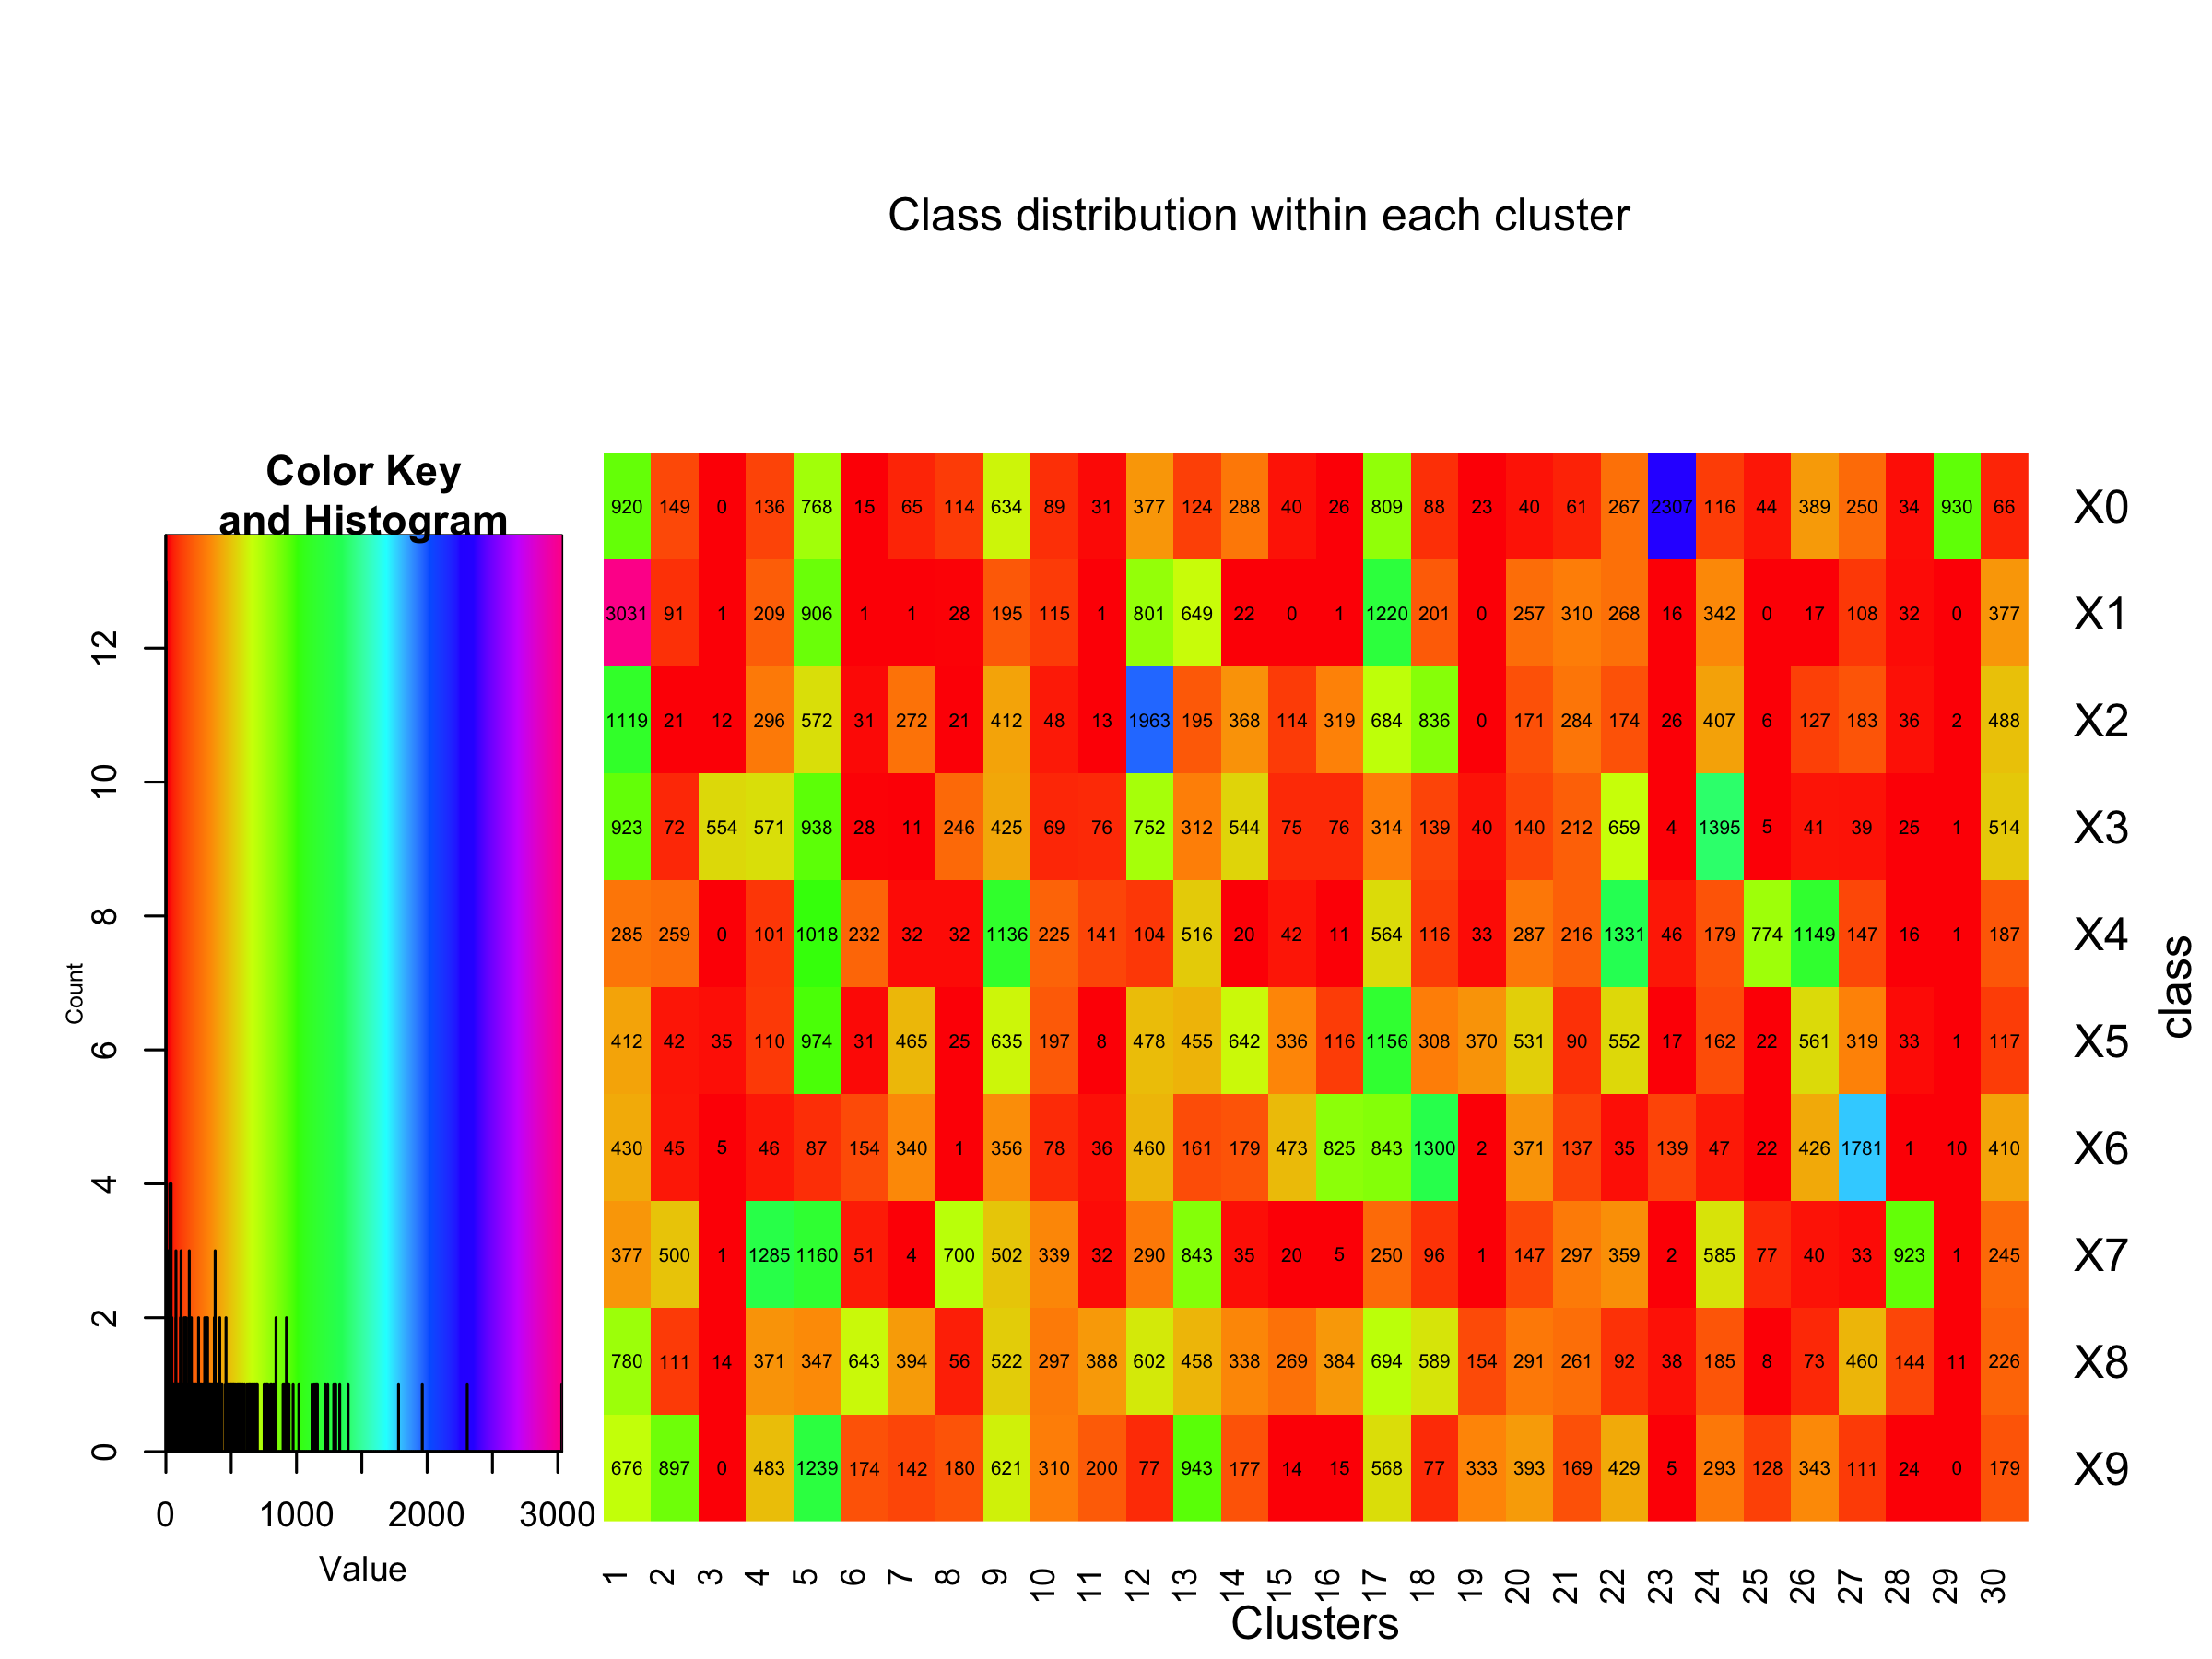
\includegraphics[width = 0.7\textwidth]{heatmap_comple.png}\label{fig:1}} 

  		\subfloat[Clustering data consiting of digit 0]{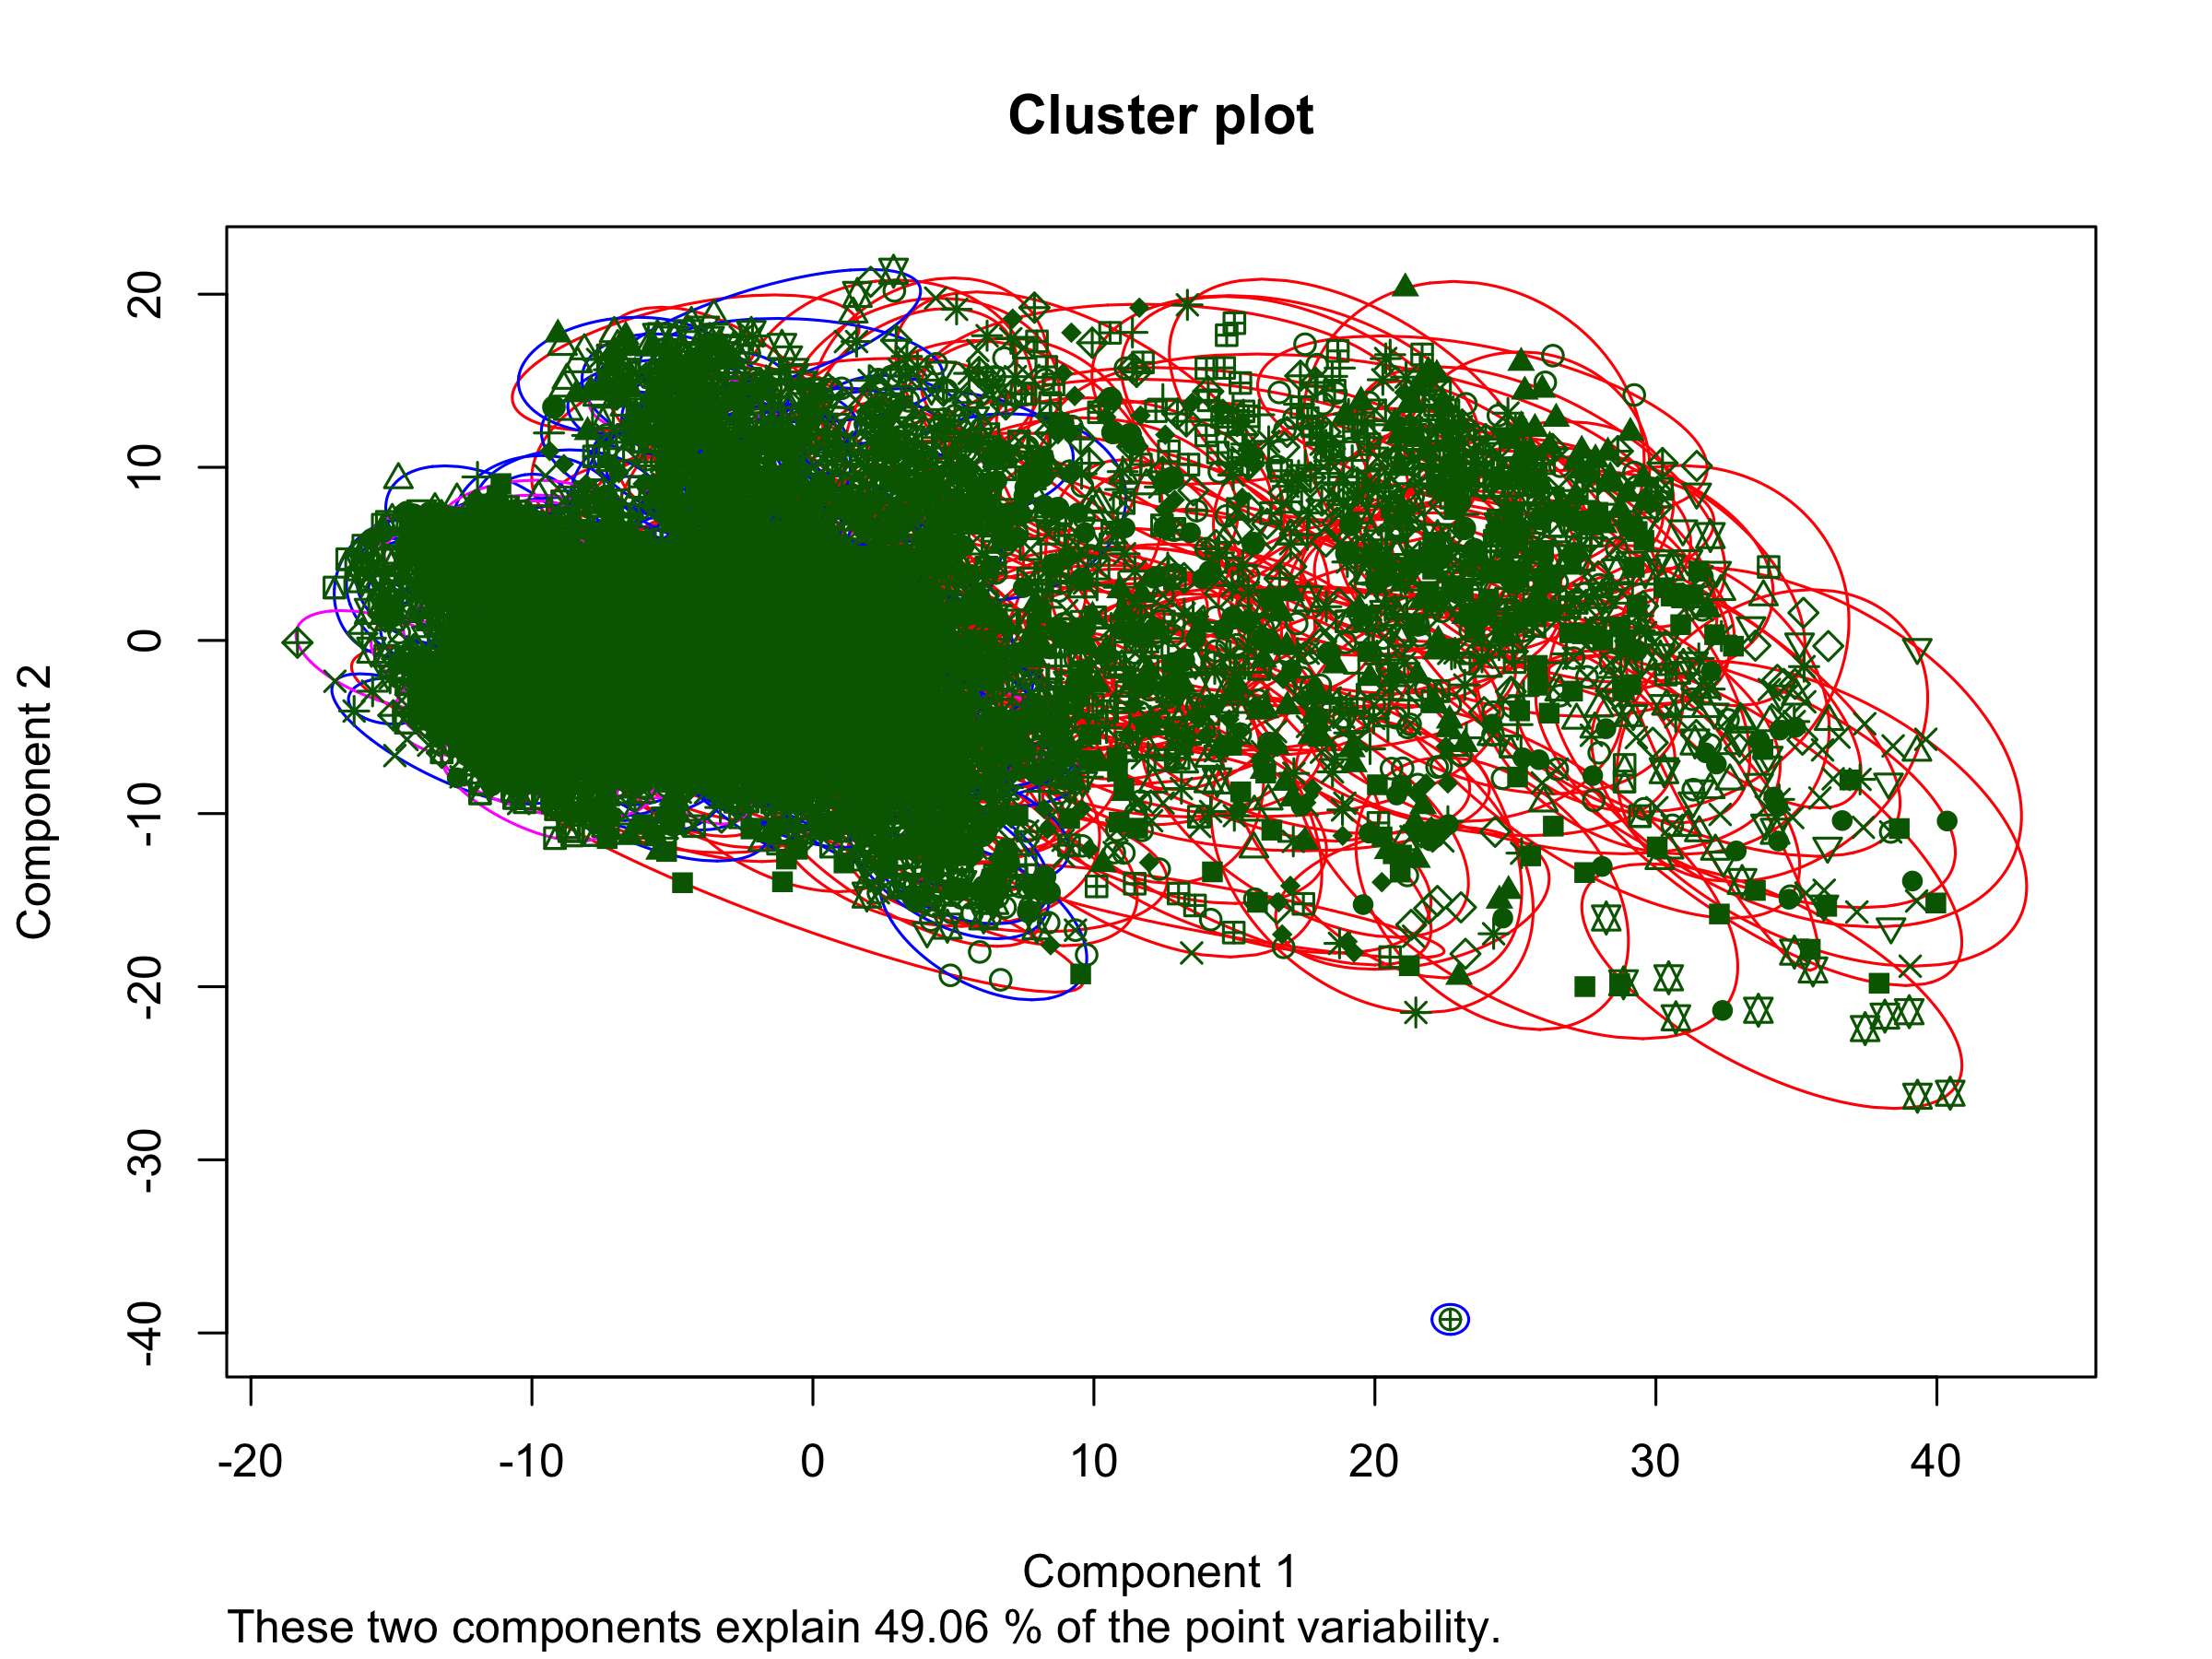
\includegraphics[width = 0.2\textwidth]{clusplot_0.png}\label{fig:2}}\hspace{1em}
%  		
  		\subfloat[Clustering data consiting of digit 1]{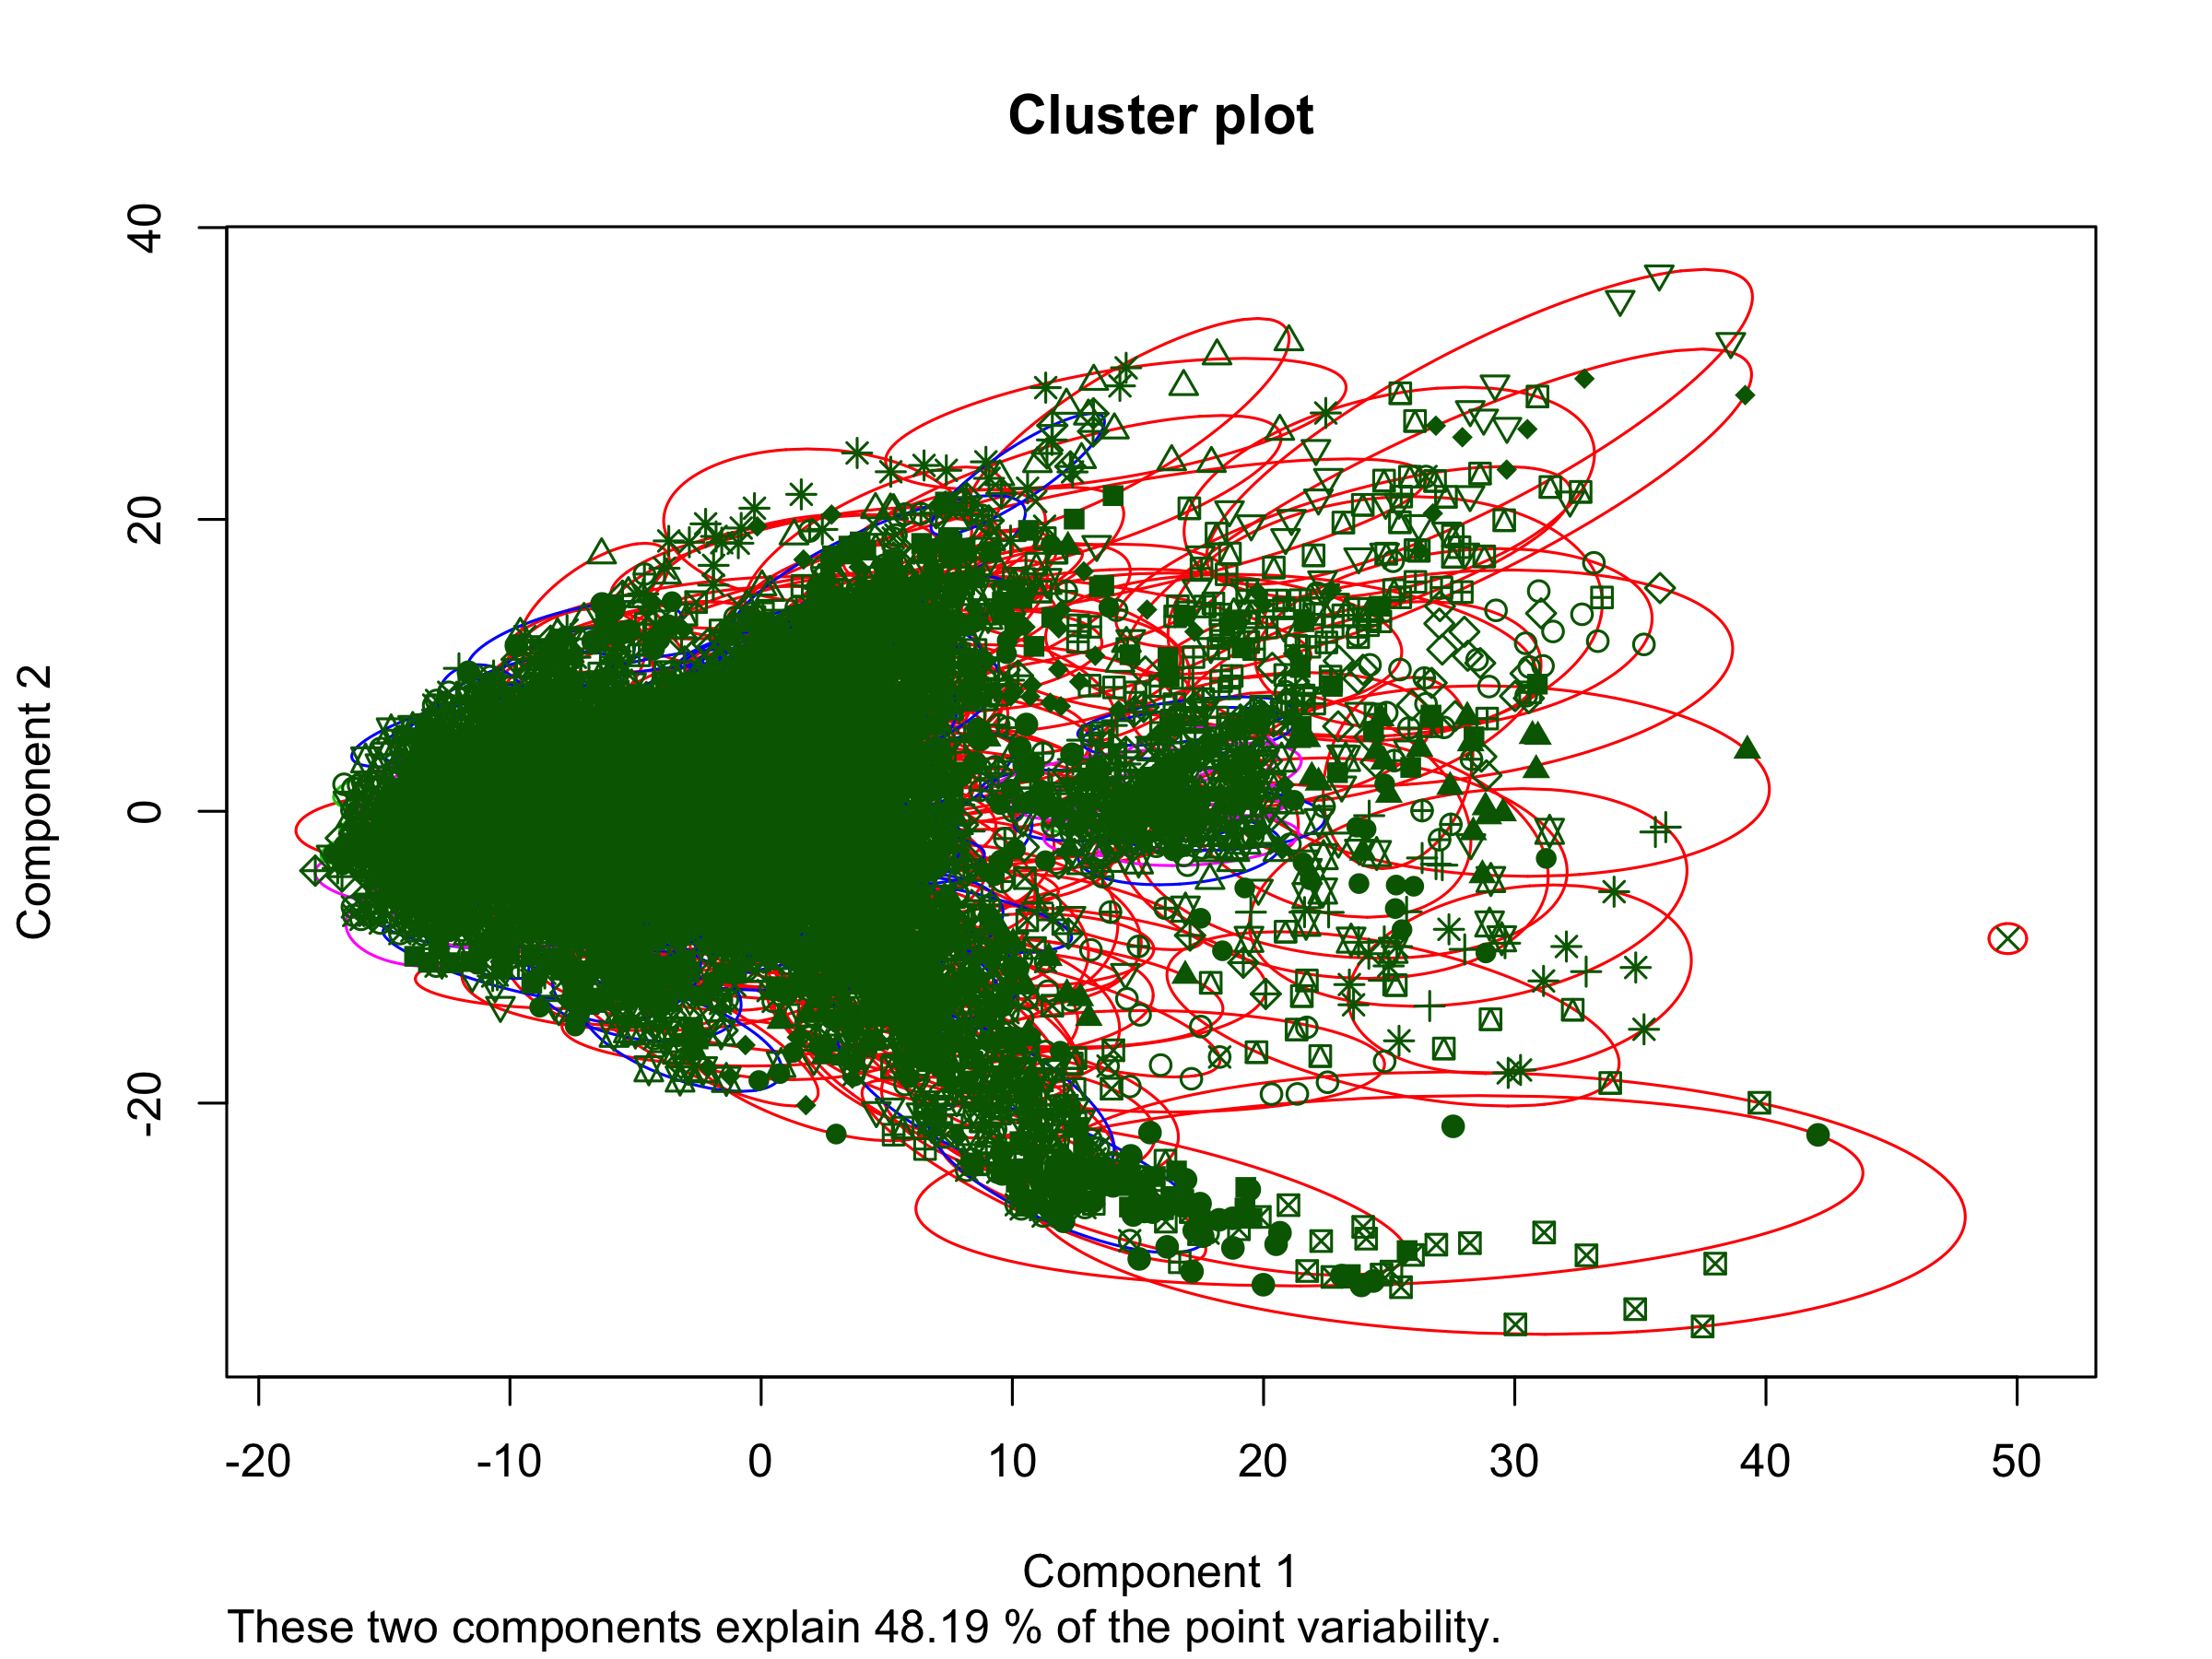
\includegraphics[width = 0.2\textwidth]{clusplot_1.png}\label{fig:3}}
%
  		\subfloat[Clustering data consiting of digit 2]{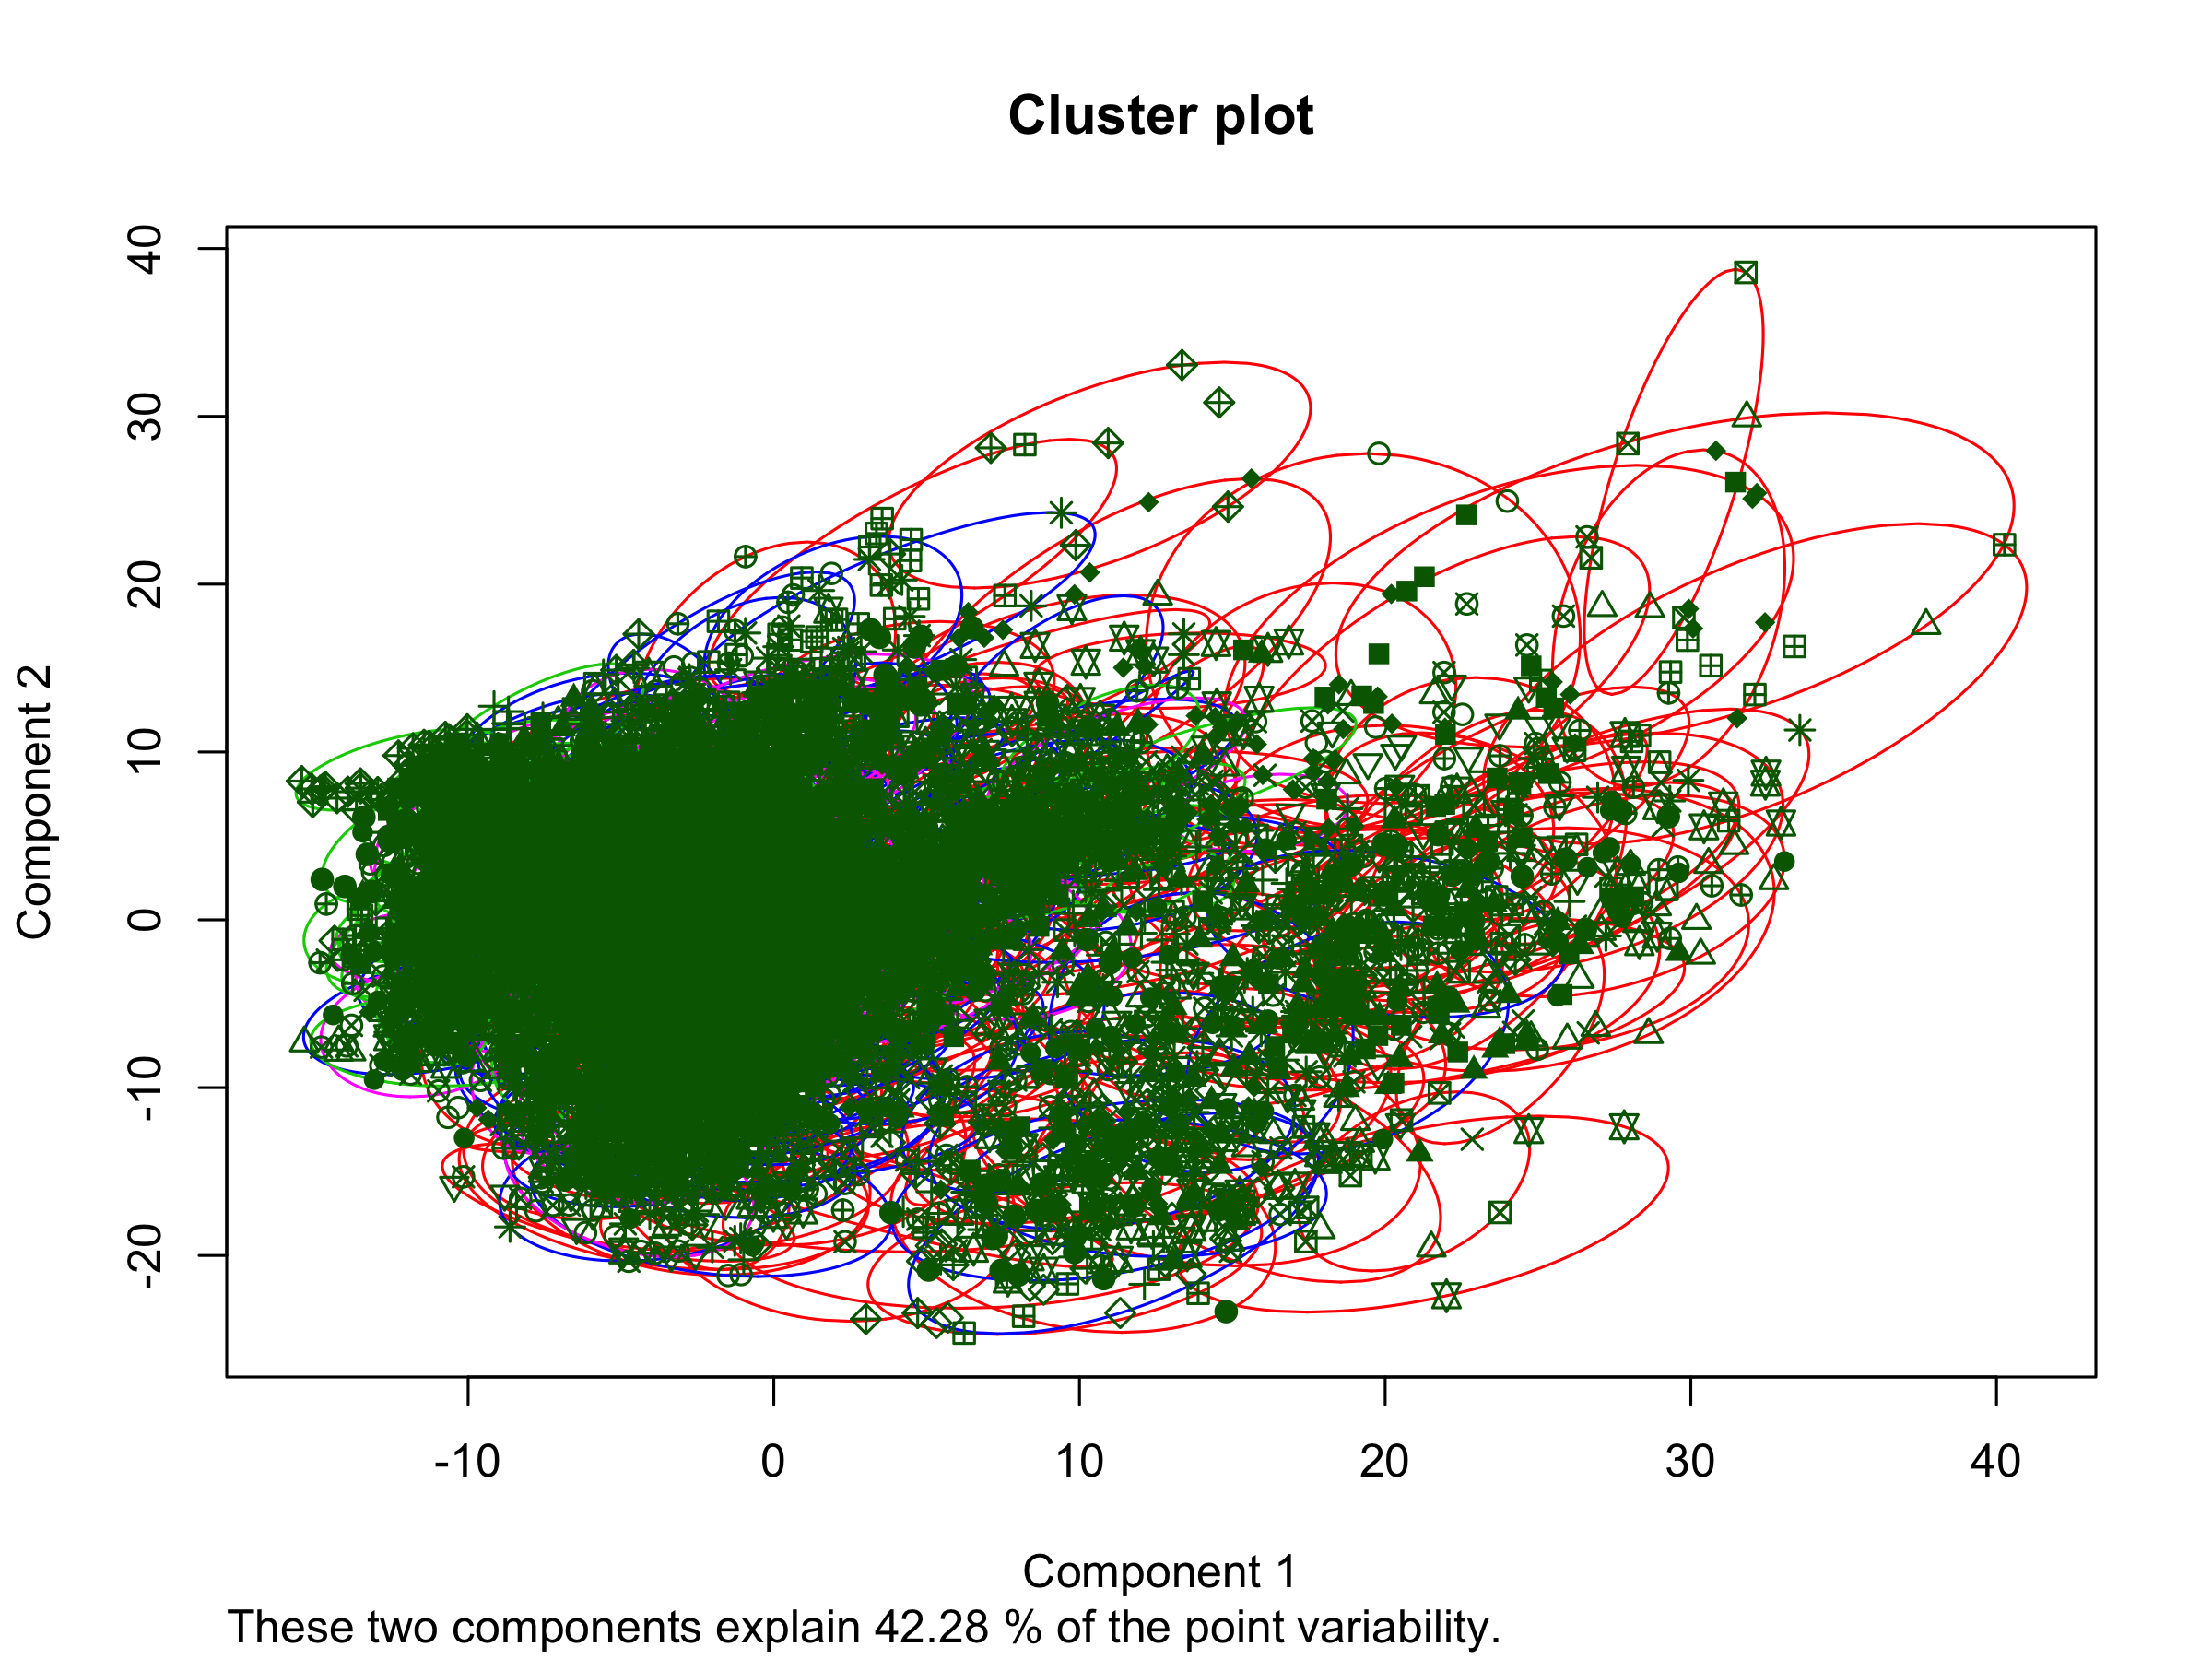
\includegraphics[width = 0.2\textwidth]{clusplot_2.png}}
%  		
  		\subfloat[Clustering data consiting of digit 3]{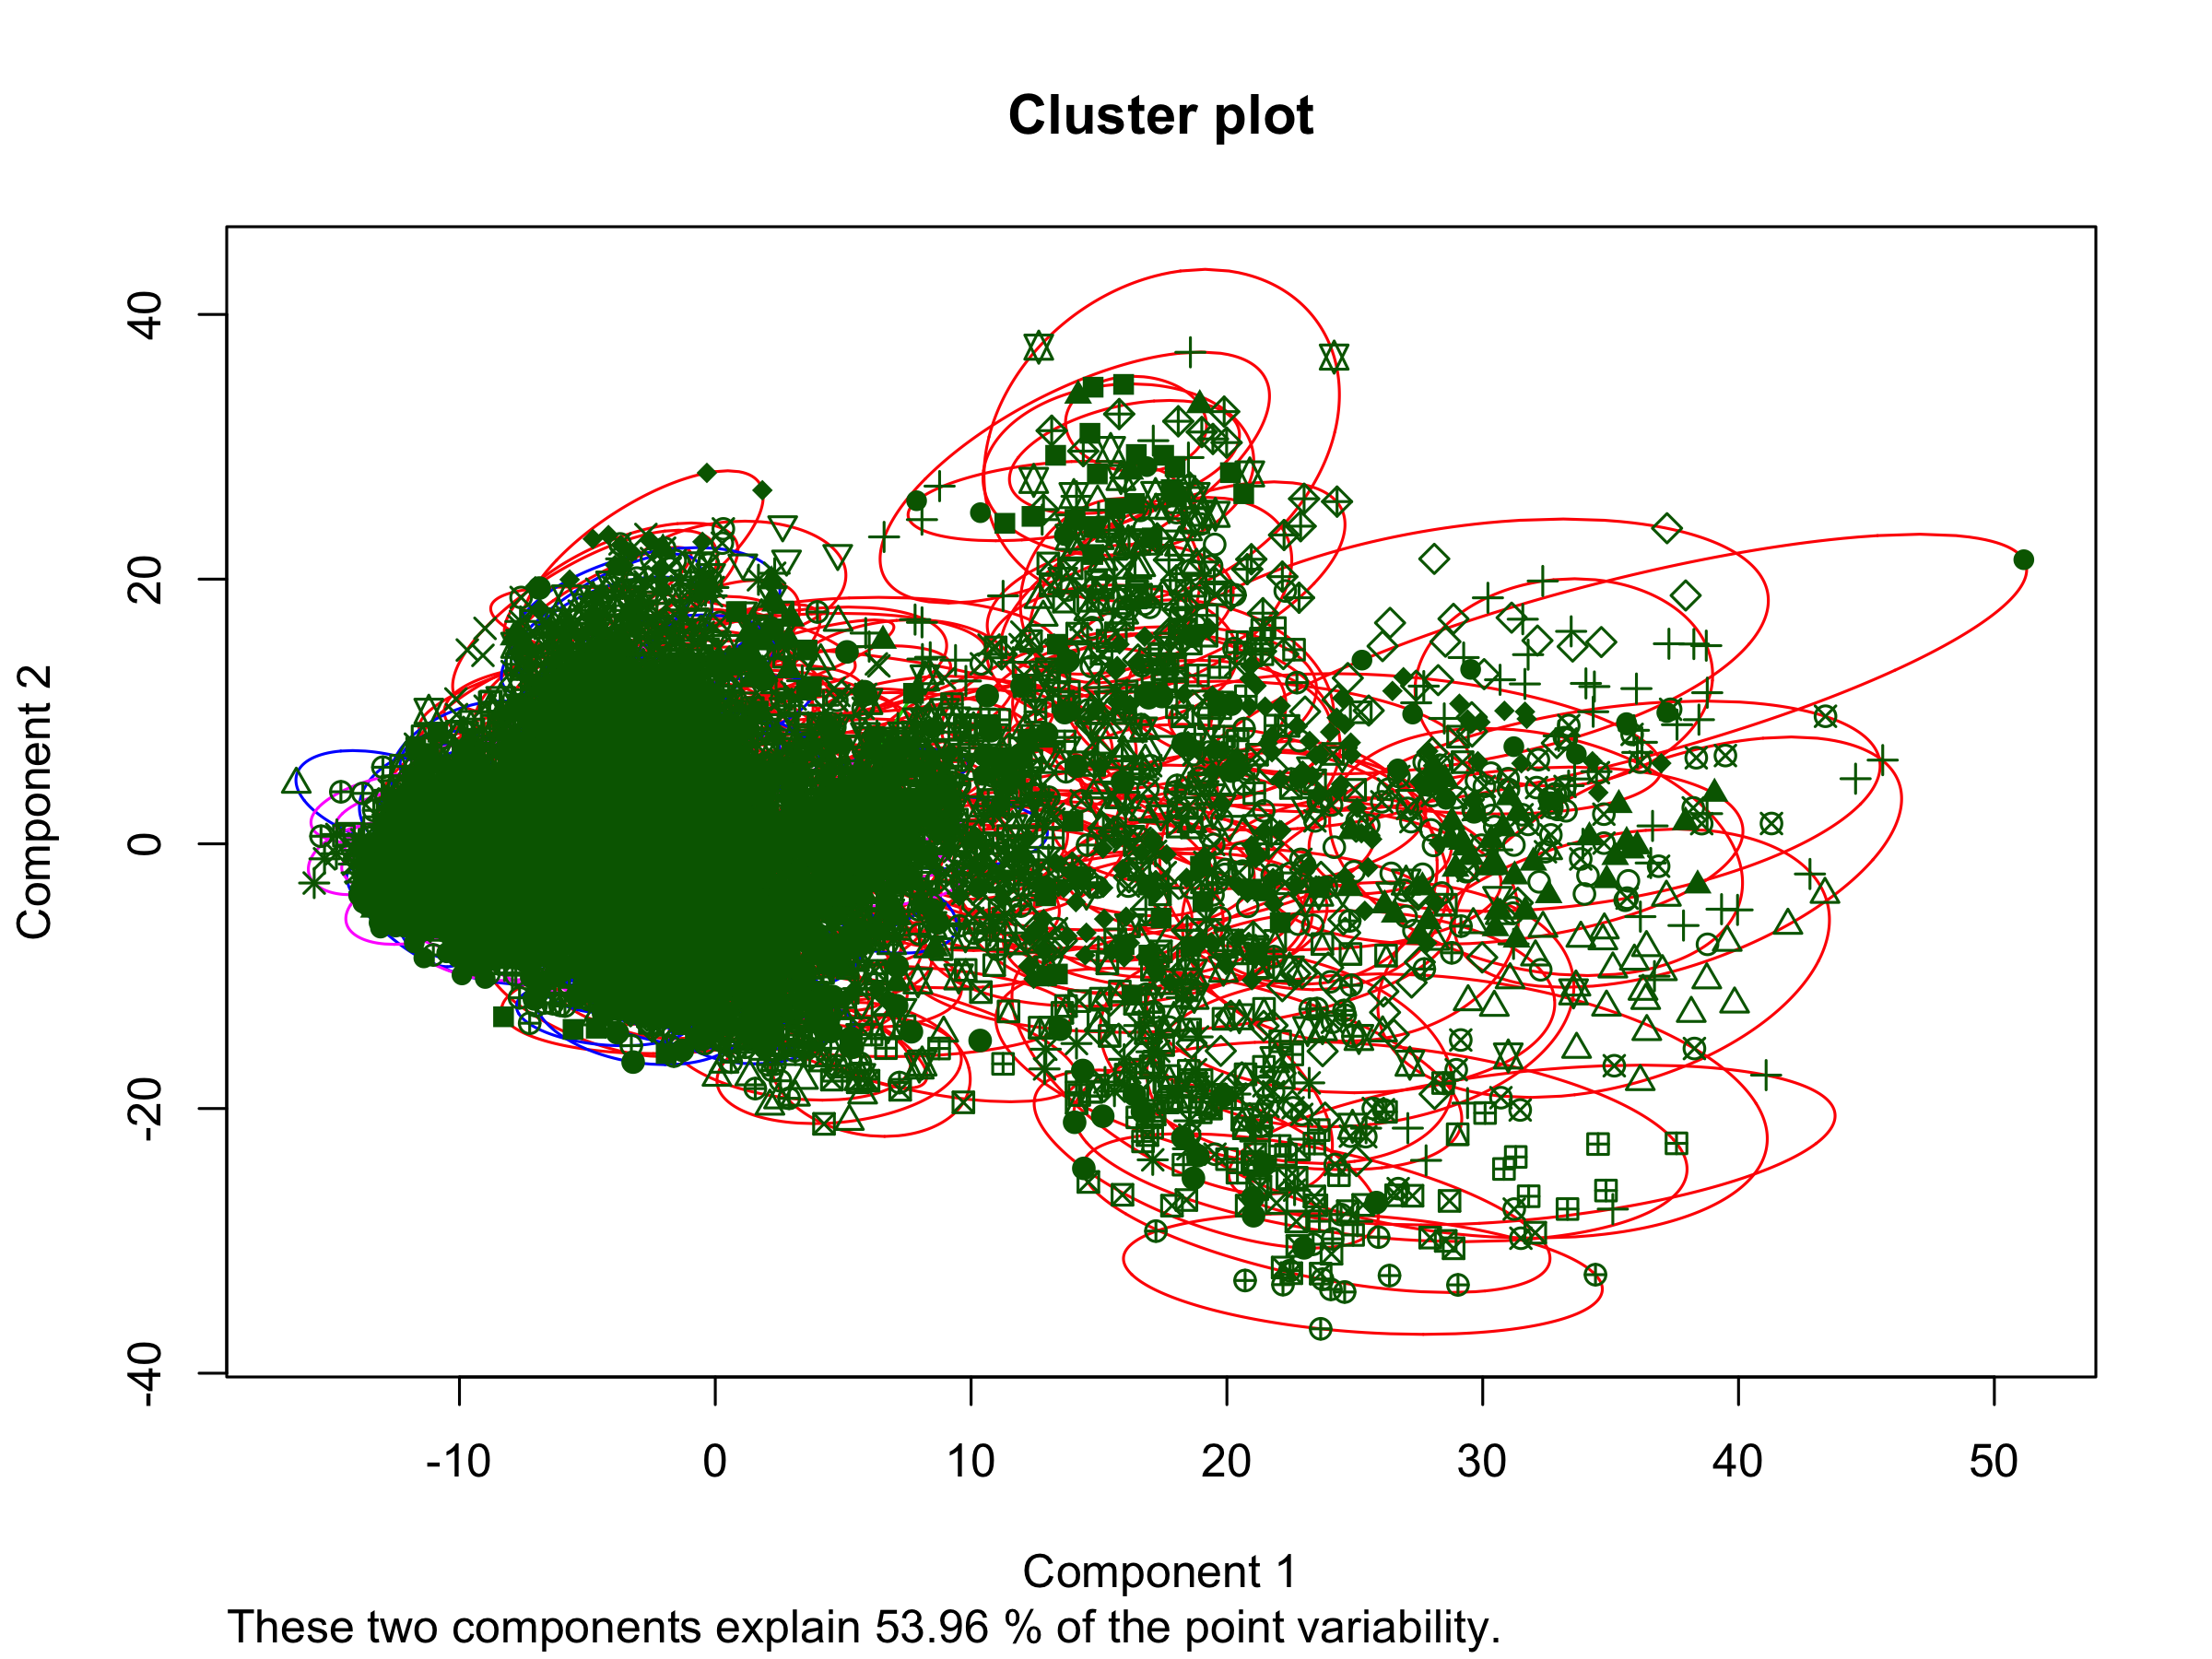
\includegraphics[width = 0.2\textwidth]{clusplot_3.png}\label{fig:2}}\hspace{1em}
%  		
%  		
  		\subfloat[Clustering data consiting of digit 4]{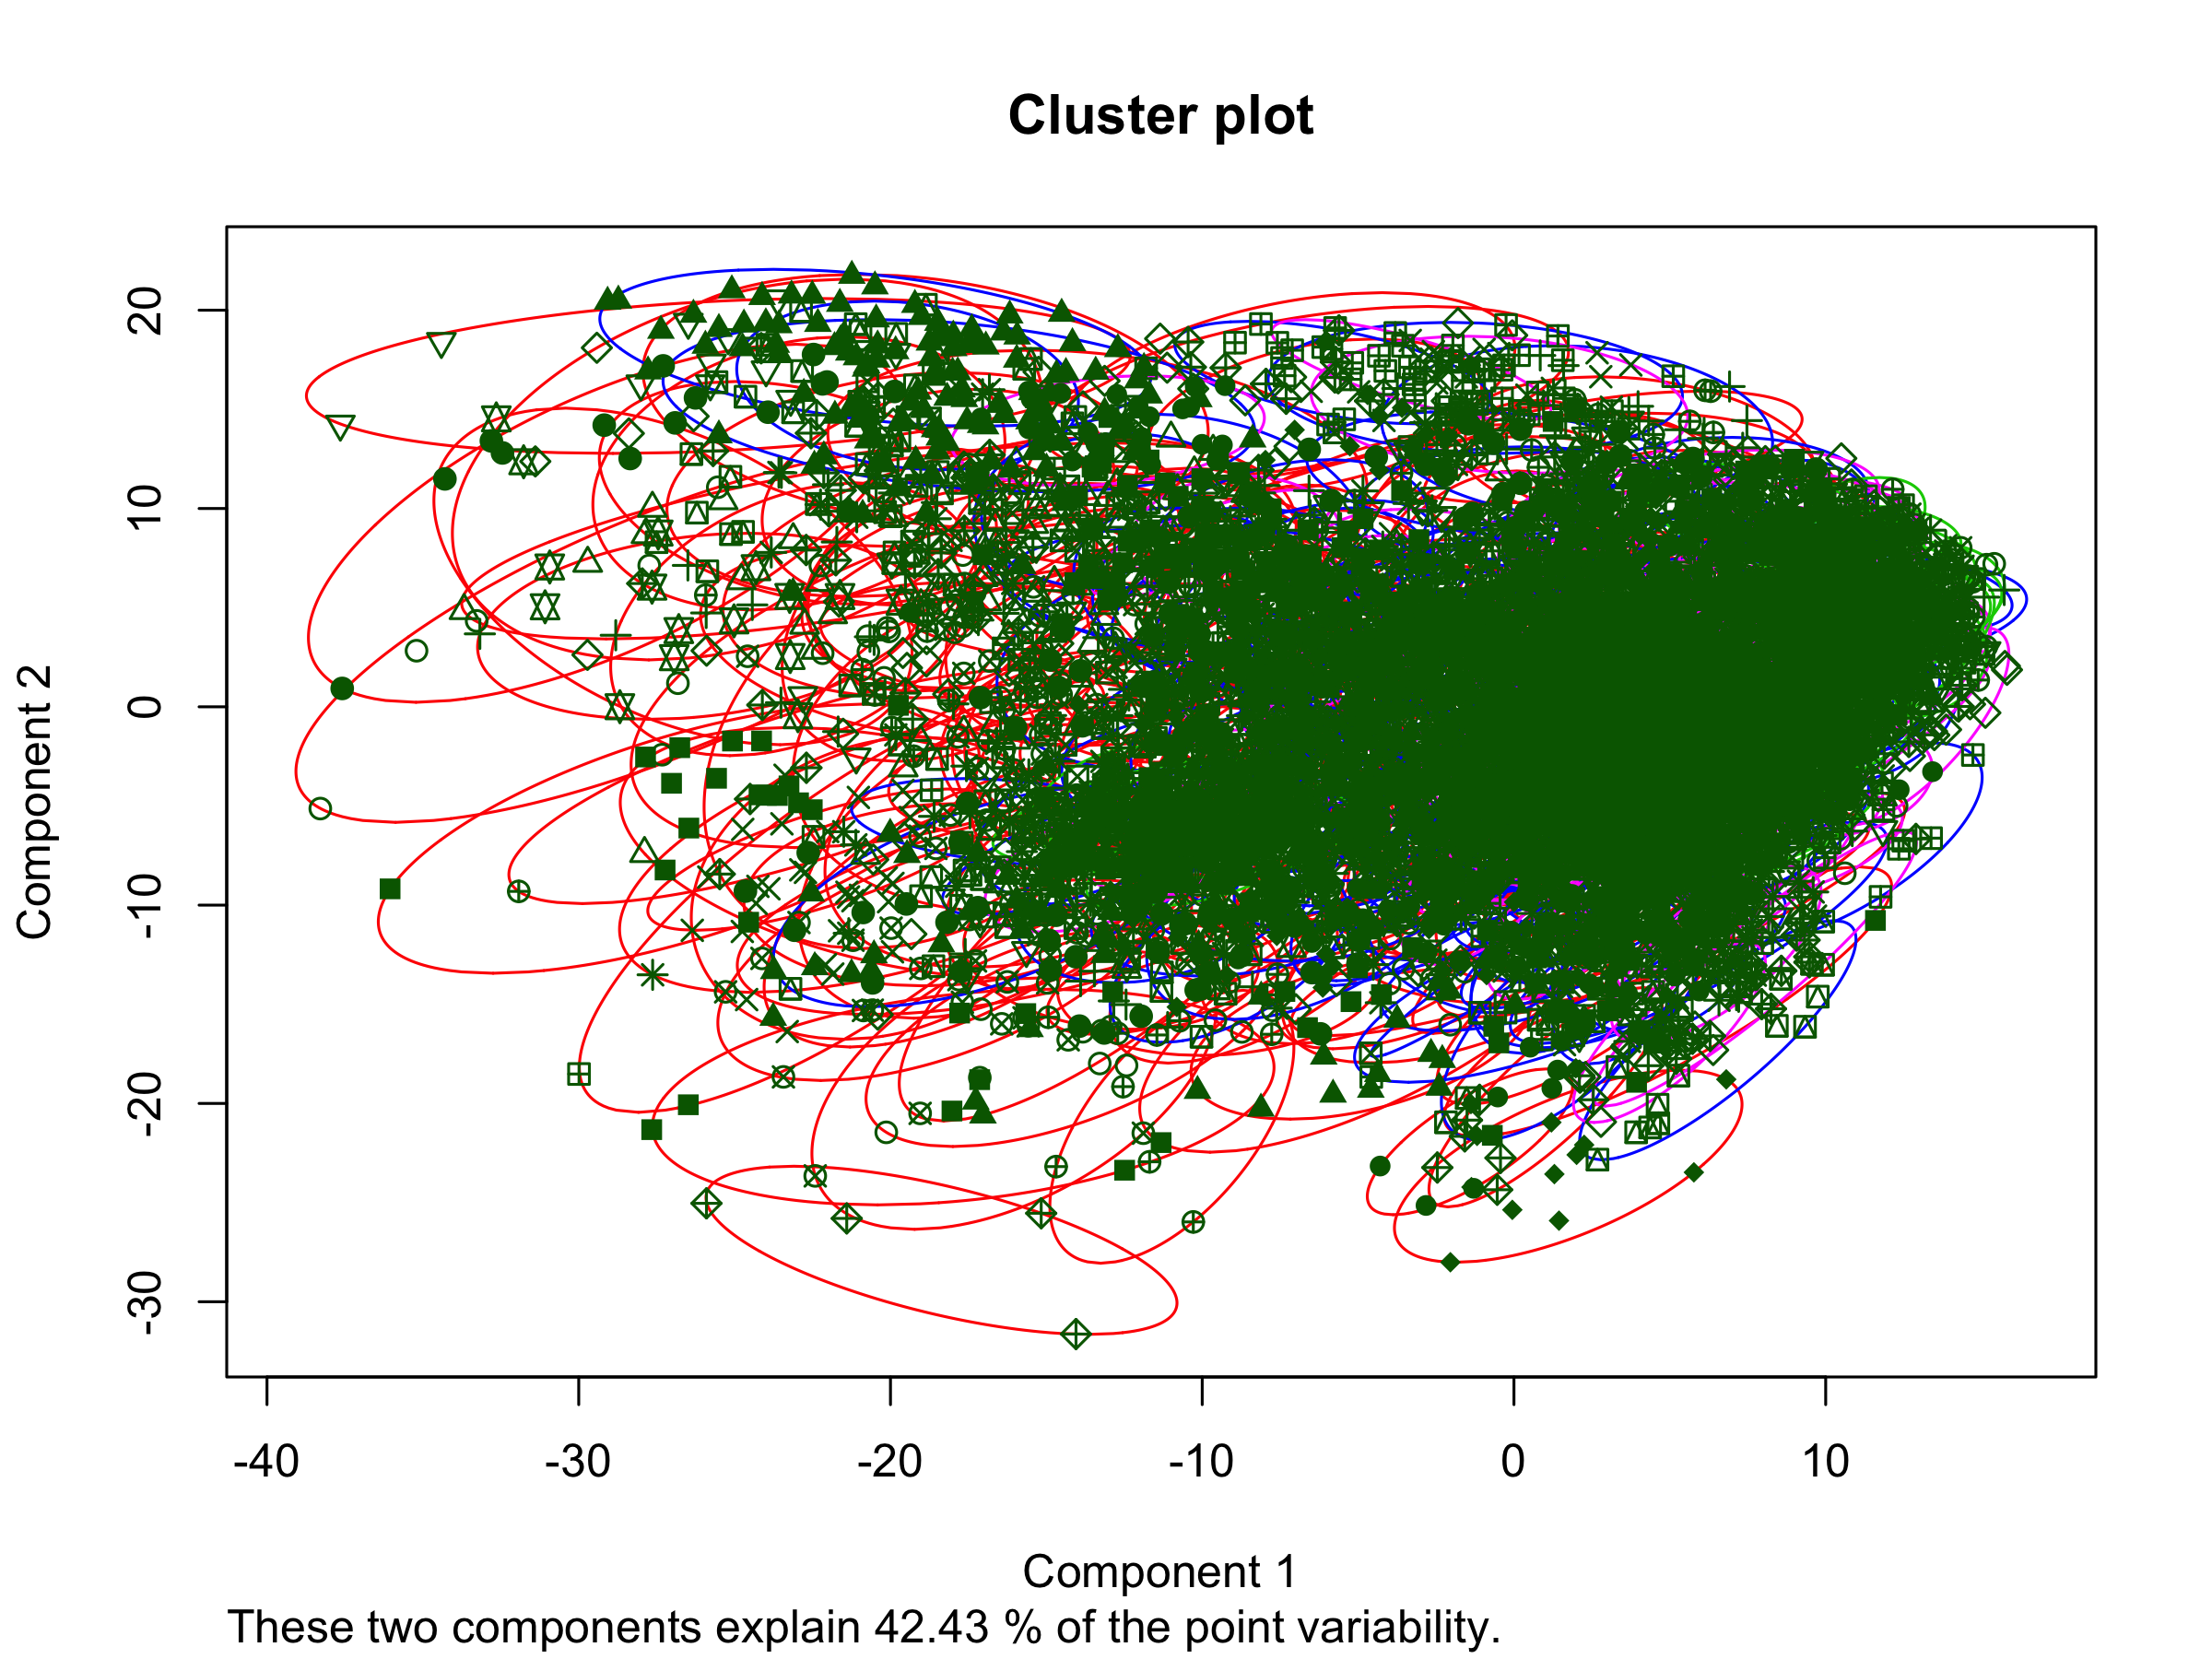
\includegraphics[width = 0.2\textwidth]{clusplot_4.png}\label{fig:3}}
%  		
  		\subfloat[Clustering data consiting of digit 5]{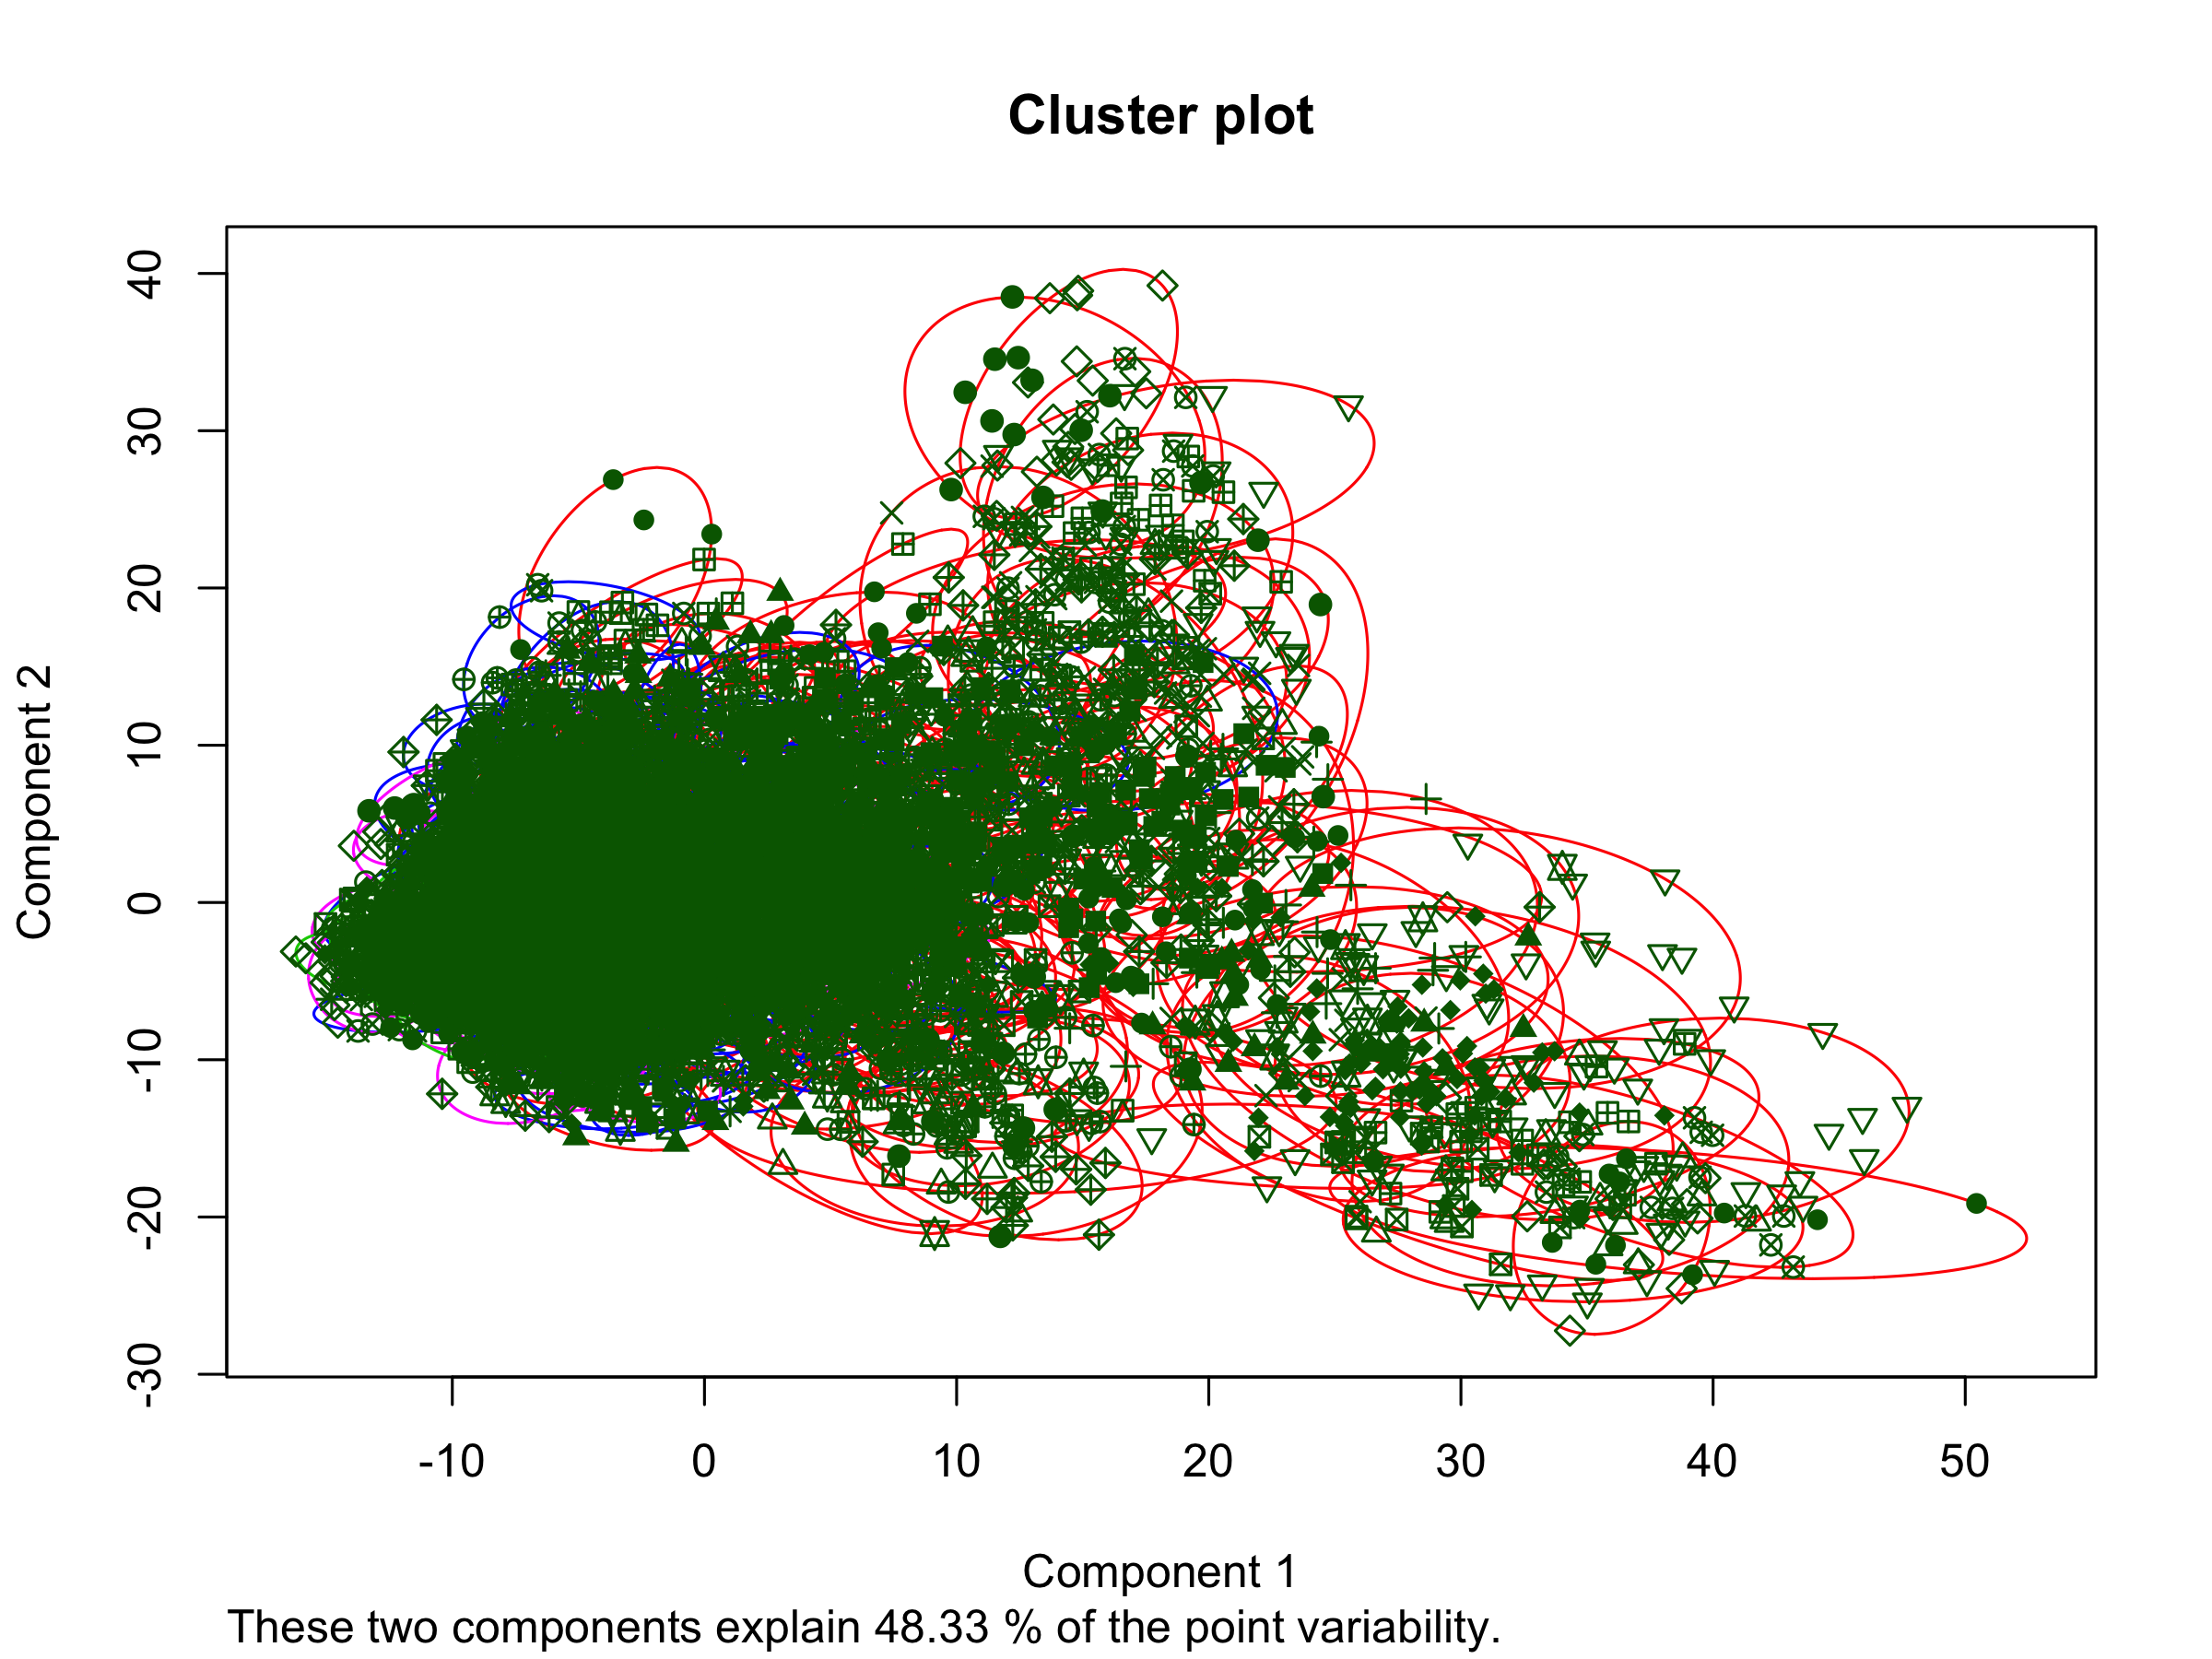
\includegraphics[width = 0.2\textwidth]{clusplot_5.png}}
%  			
%  			
 		\subfloat[Clustering data consiting of digit 6]{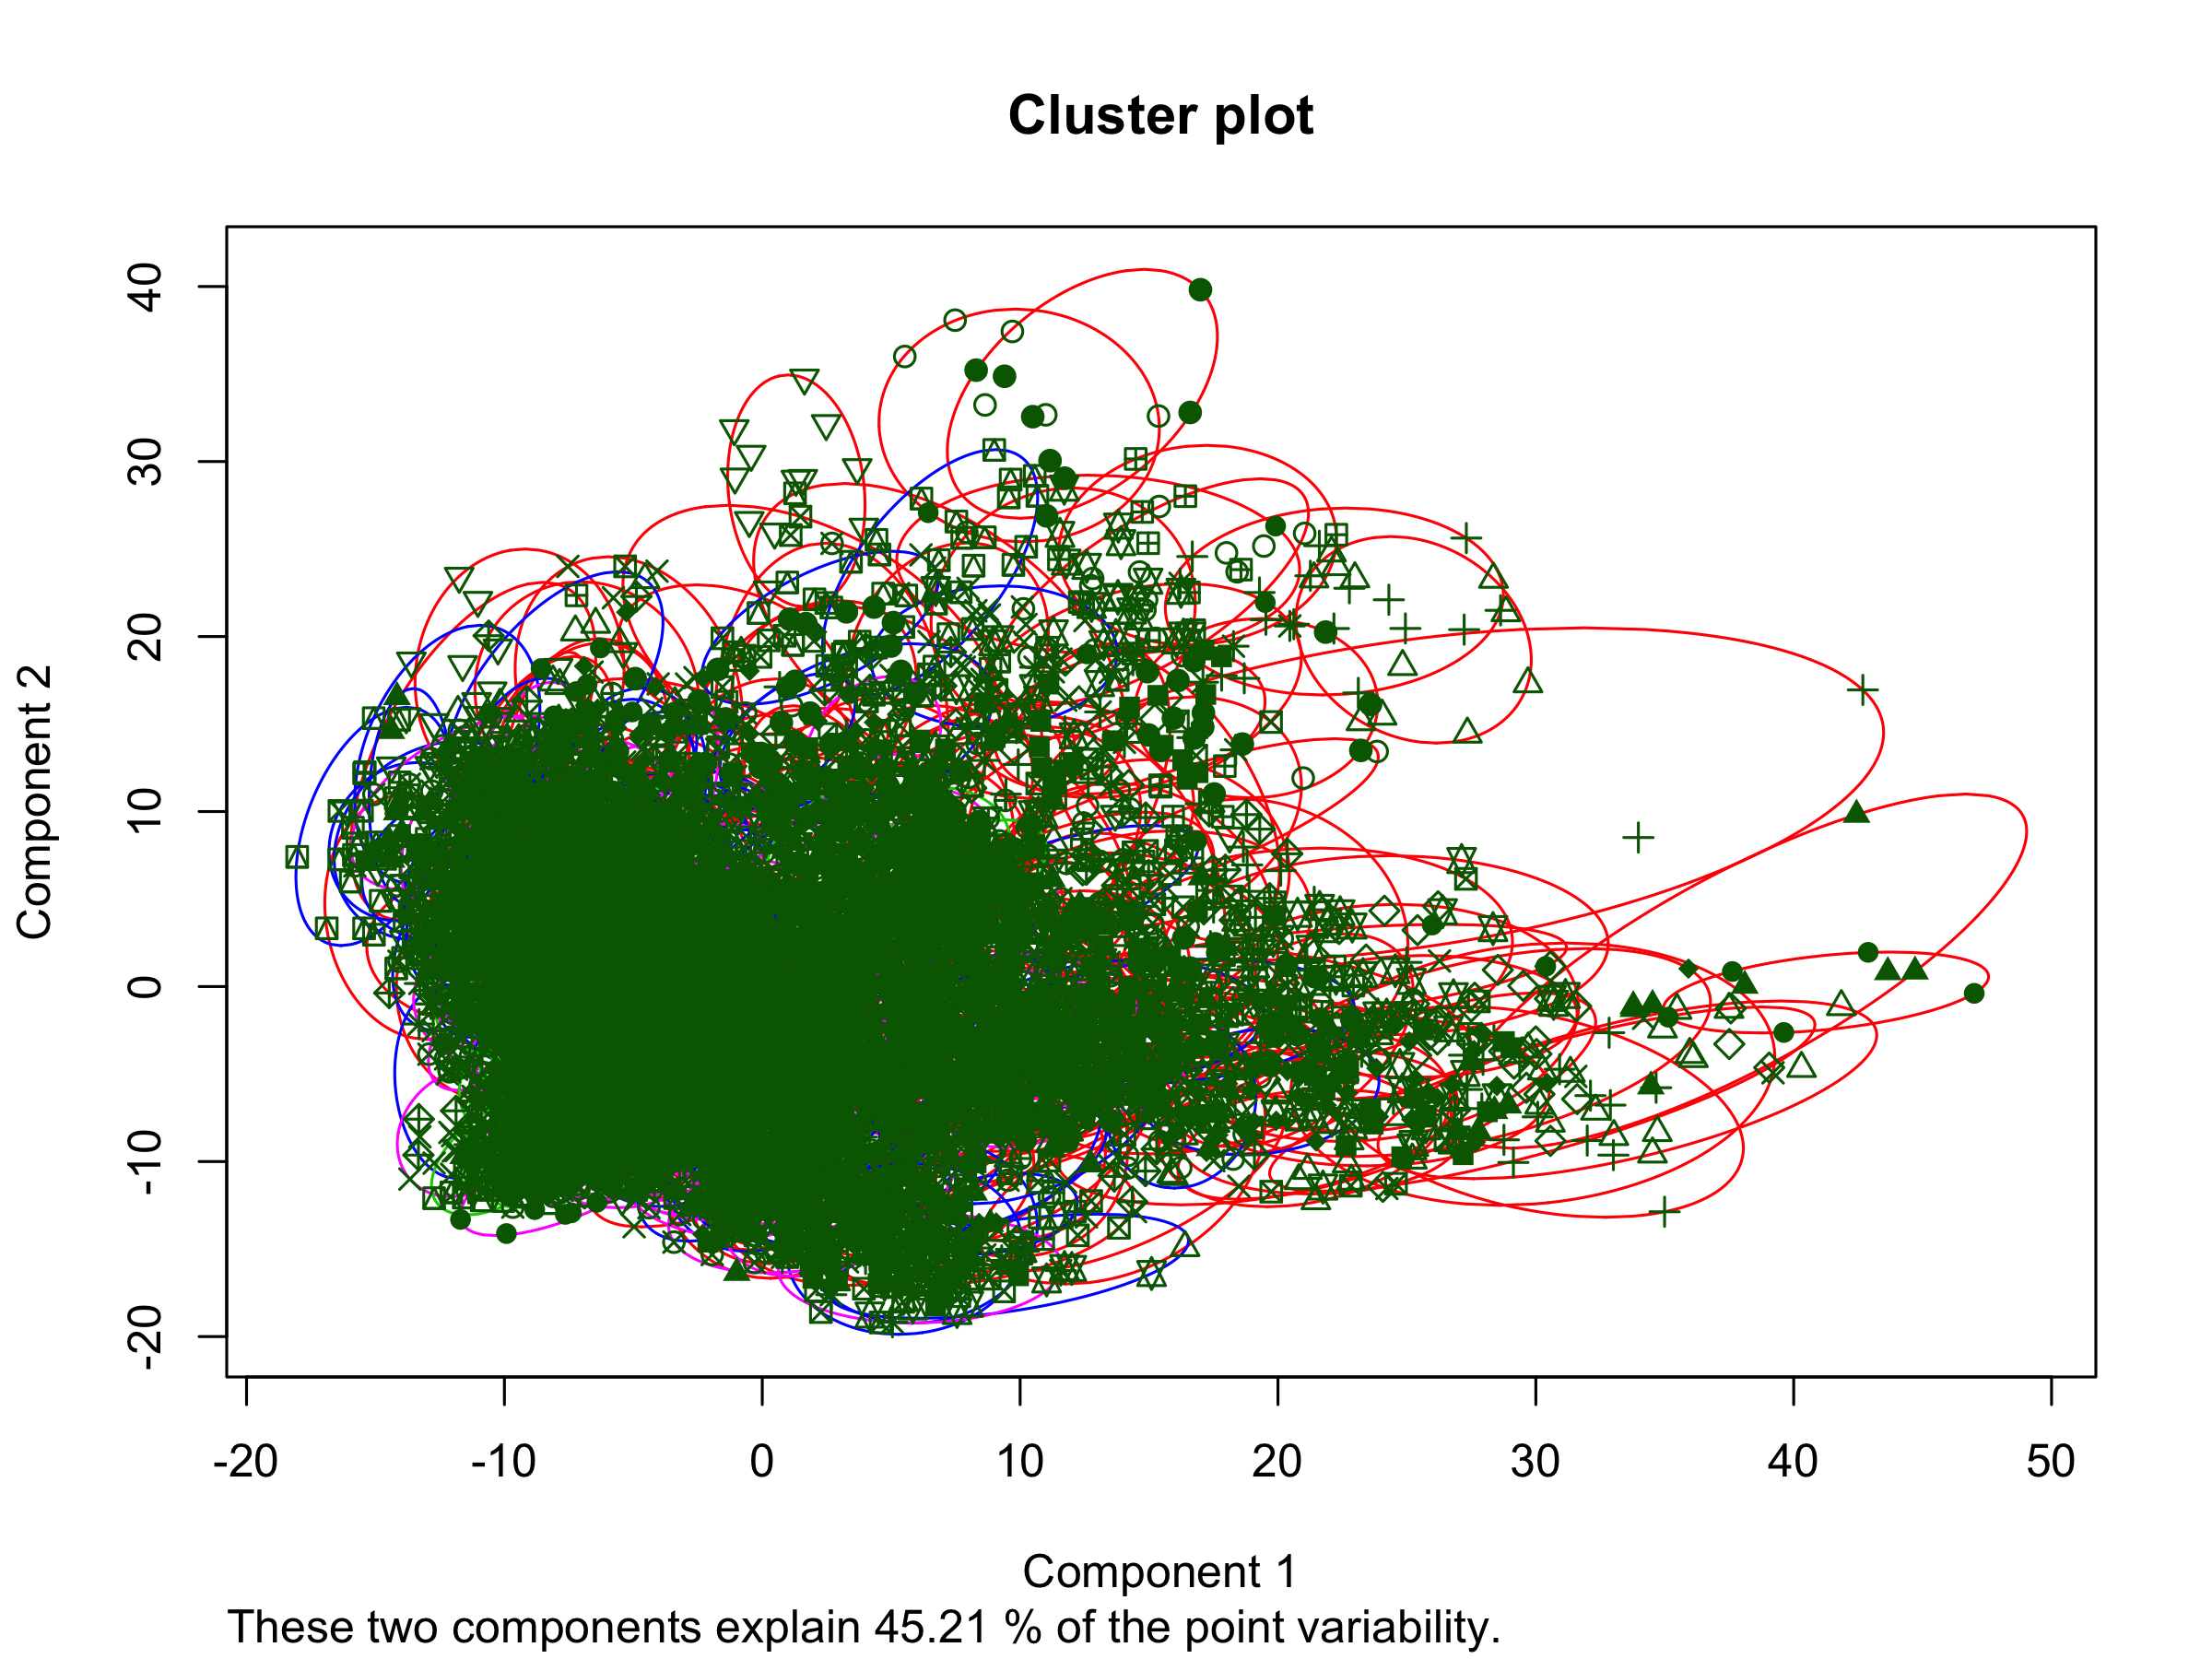
\includegraphics[width = 0.2\textwidth]{clusplot_6.png}\label{fig:2}}\hspace{1em}
%%  		
%%  		
  		\subfloat[Clustering data consiting of digit 7]{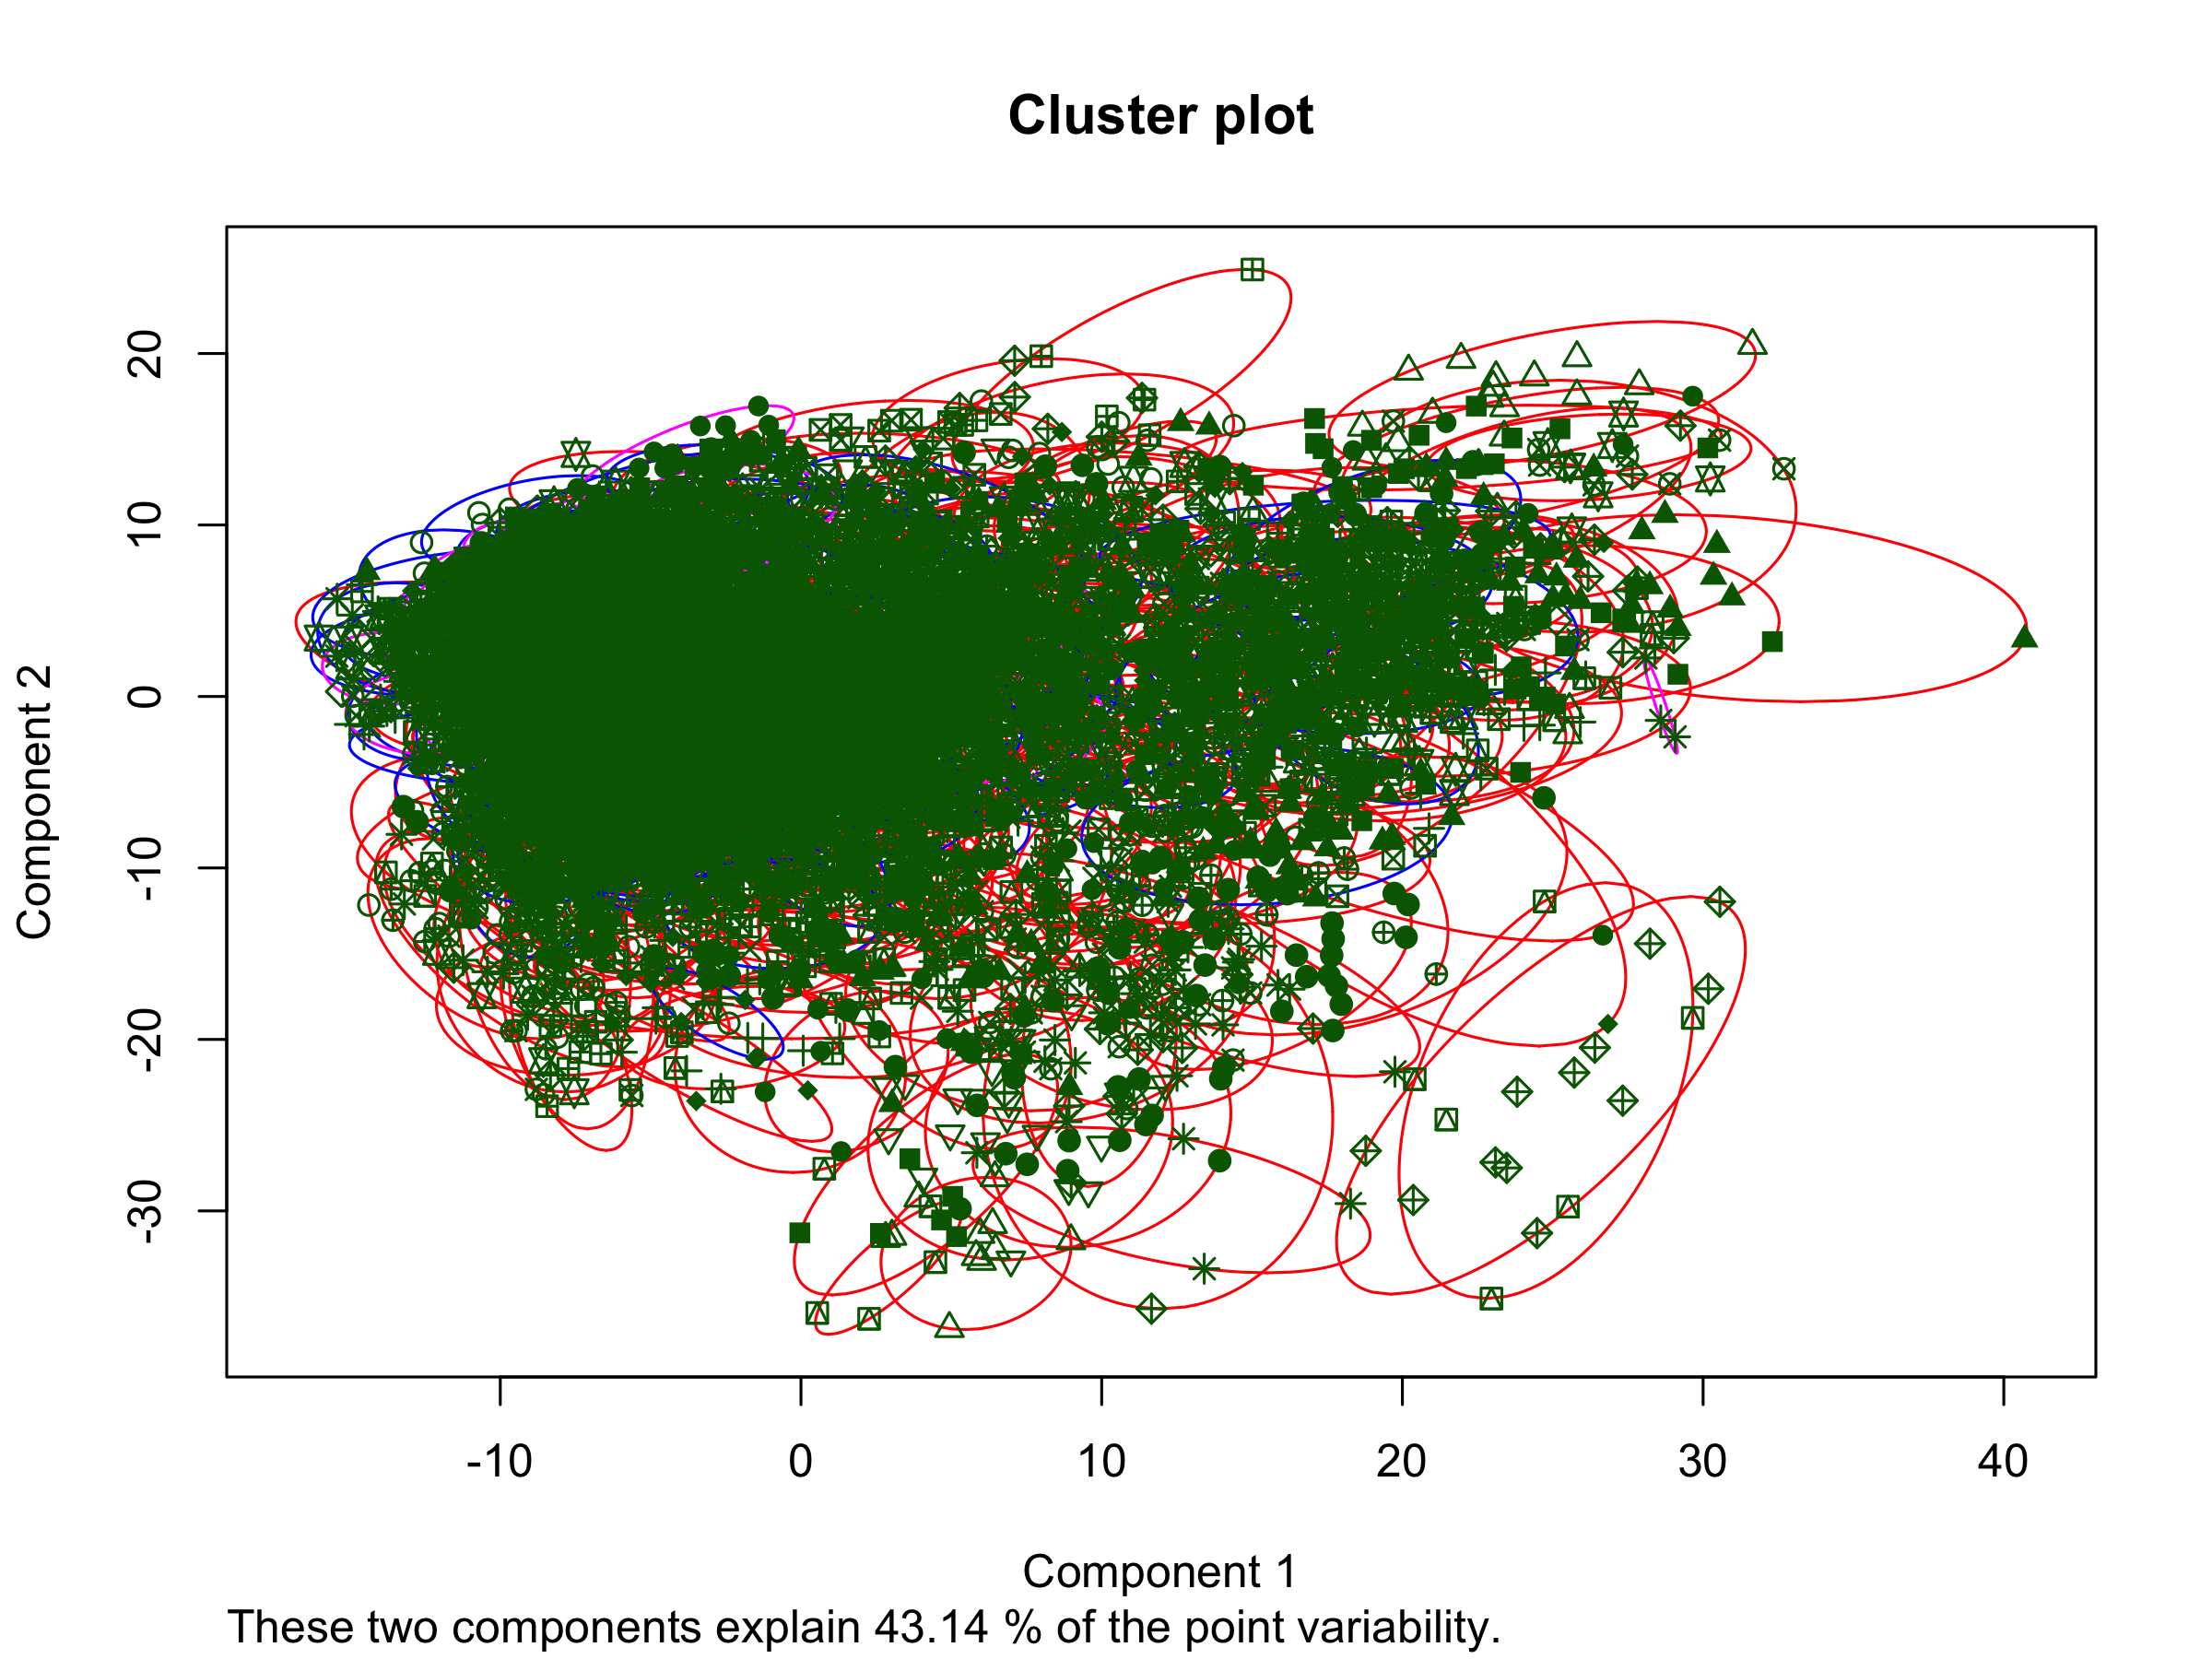
\includegraphics[width = 0.2\textwidth]{clusplot_7.png}\label{fig:3}}
%%
  		\subfloat[Clustering data consiting of digit 8]{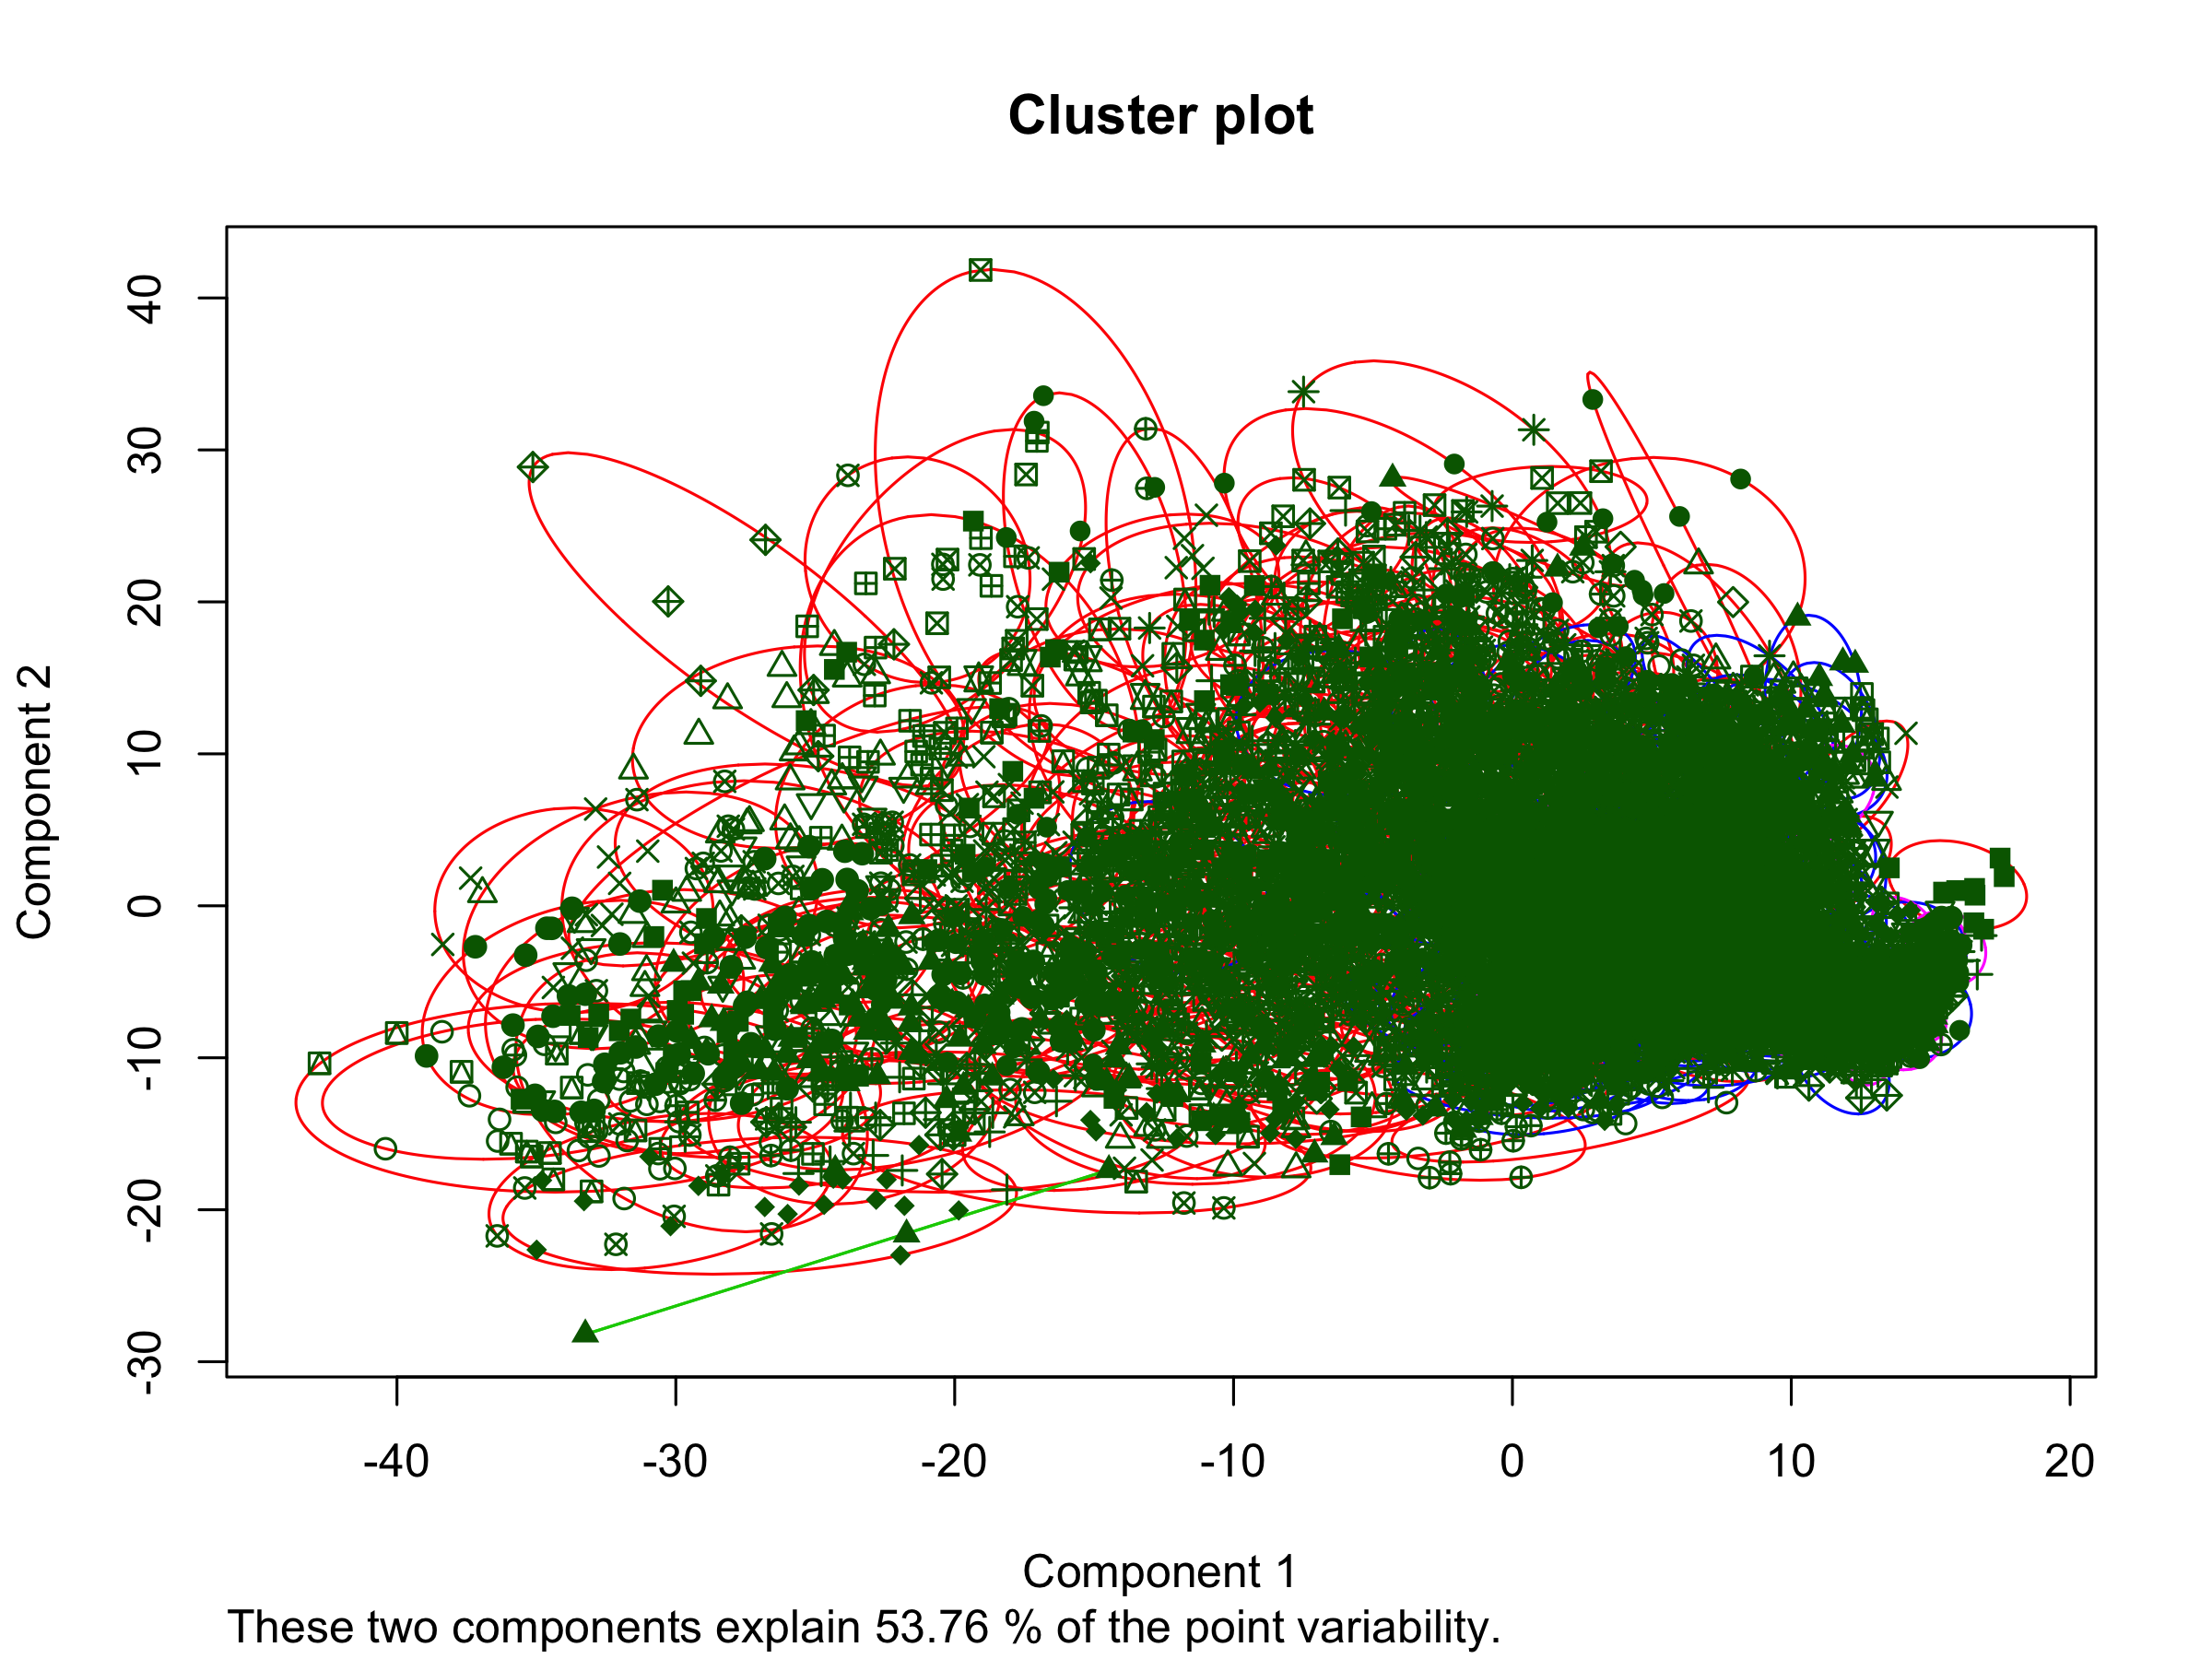
\includegraphics[width = 0.2\textwidth]{clusplot_8.png}}
%%  		 
  		 \subfloat[Clustering data consiting of digit 9]{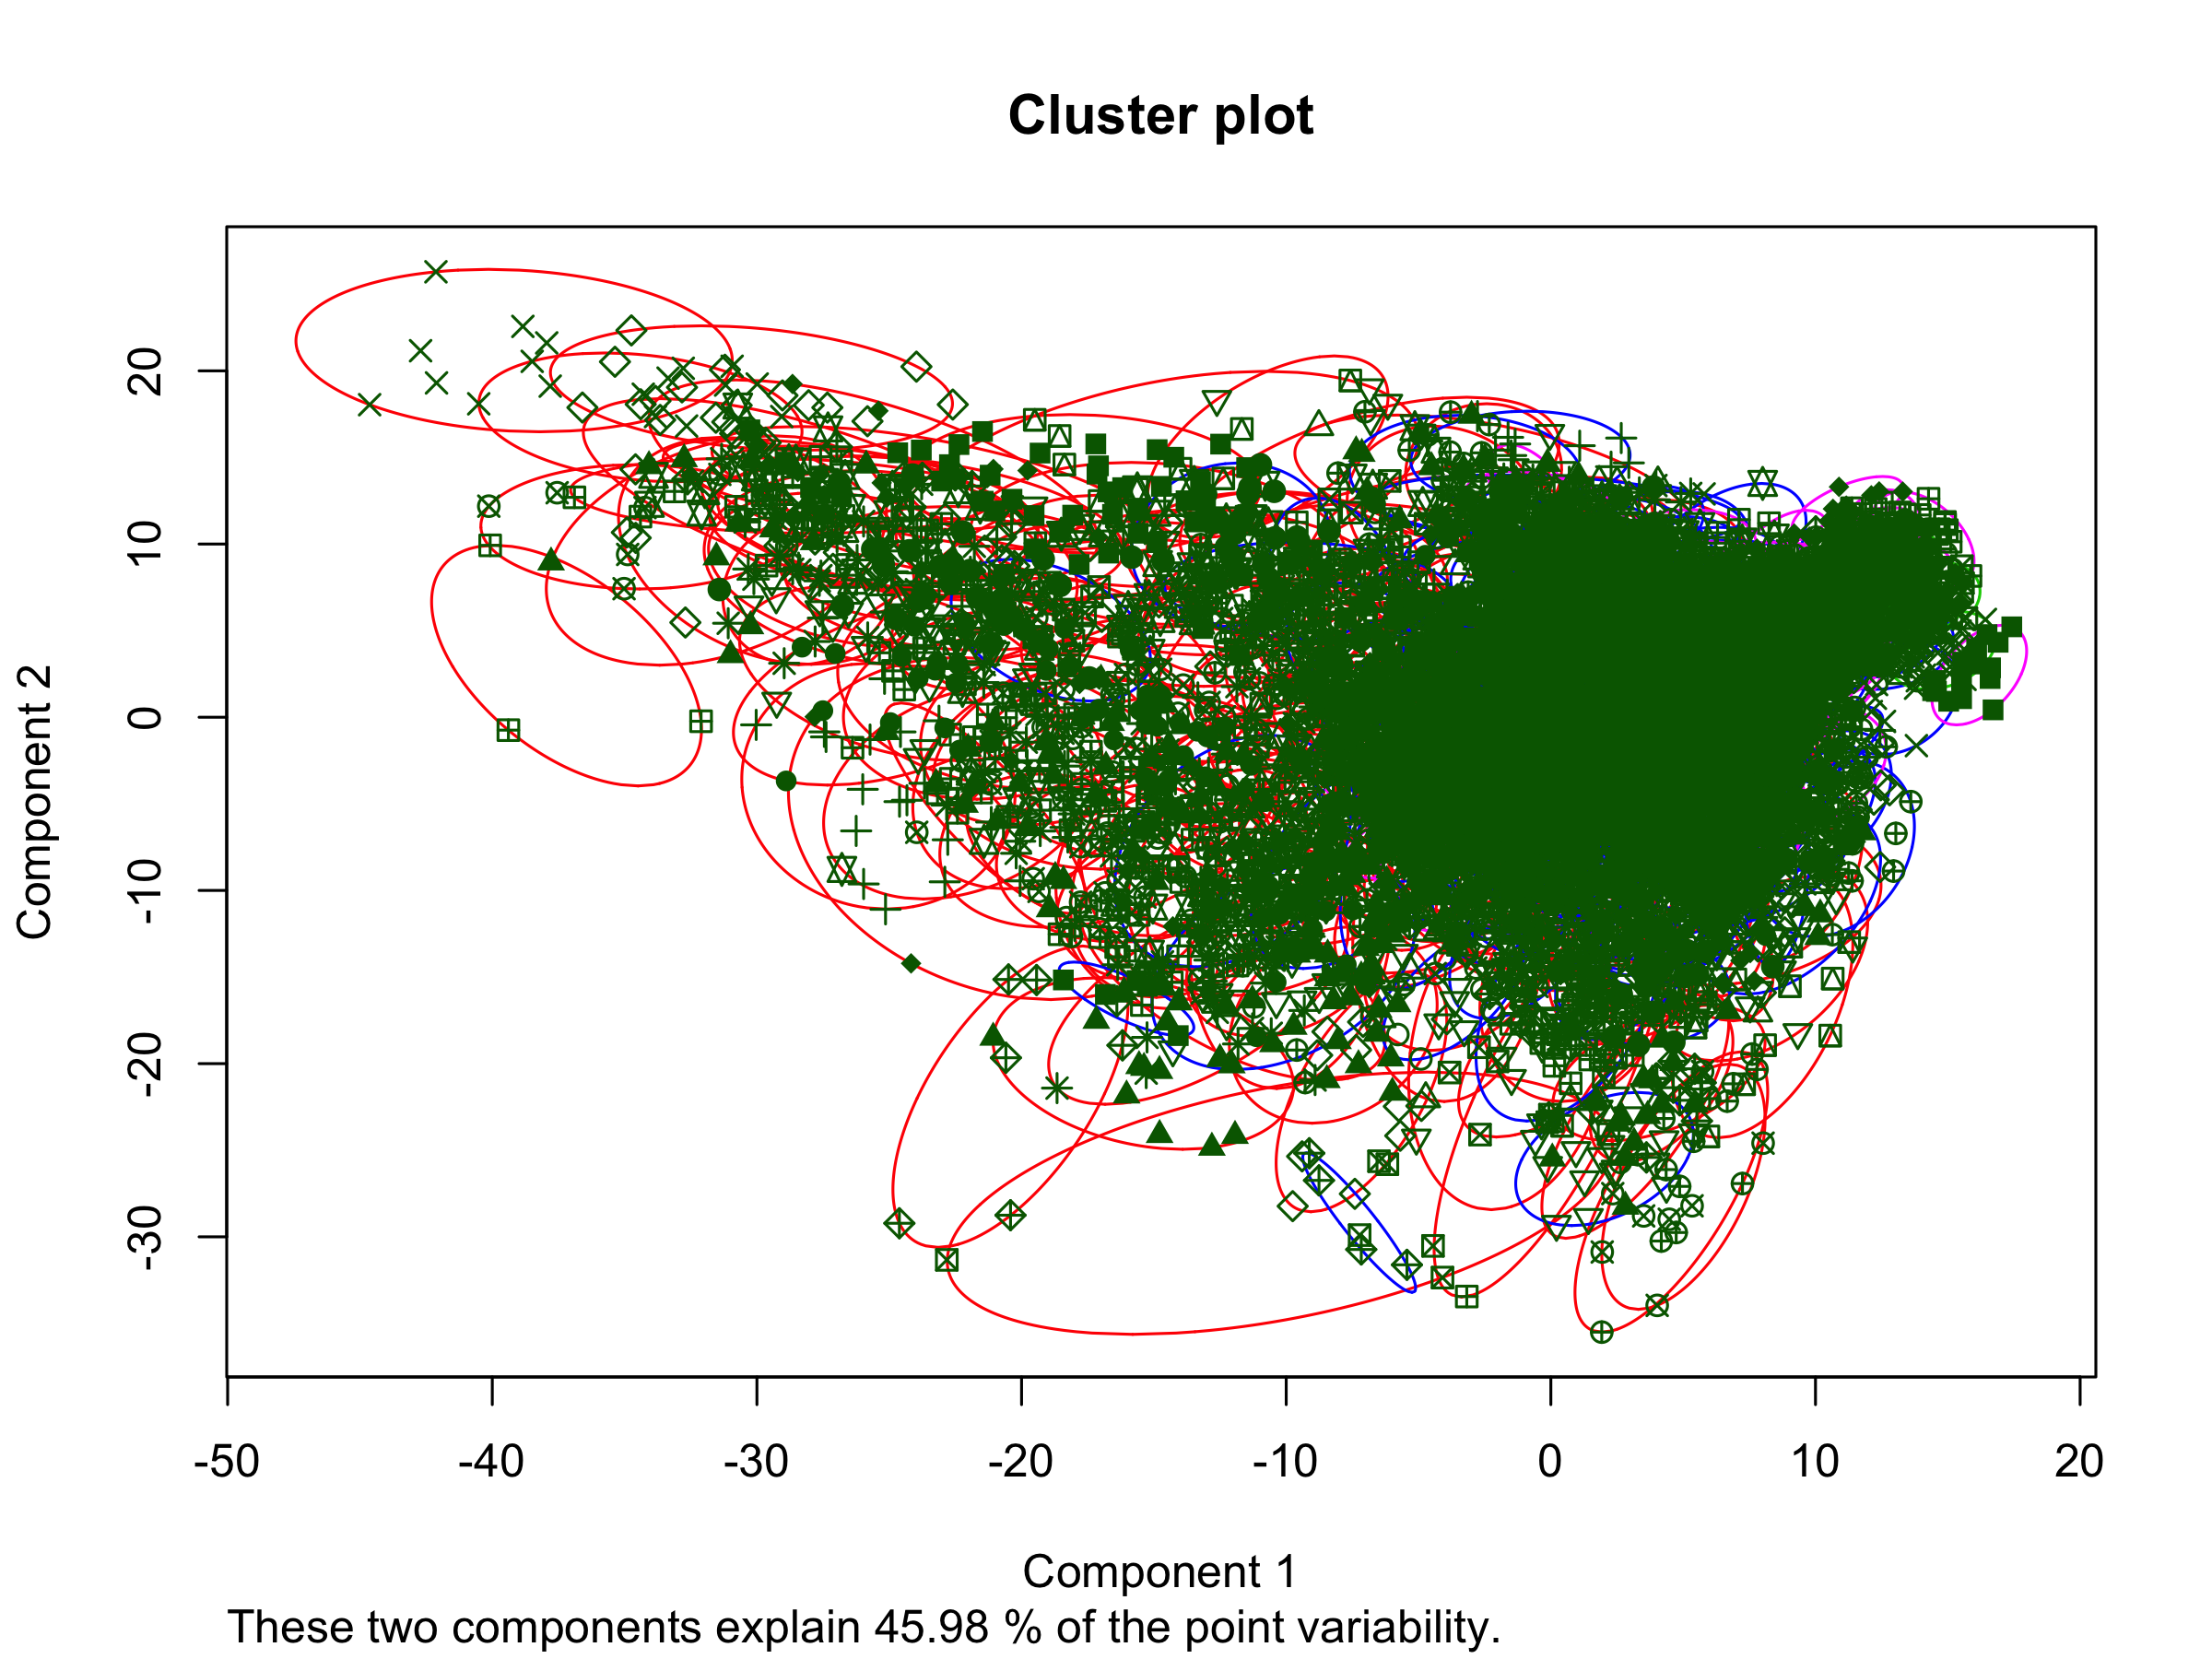
\includegraphics[width = 0.2\textwidth]{clusplot_9.png}\label{fig:2}}\hspace{1em}
  		\caption{This and that}
	\end{figure}

\todo{some text}
\todo{some text}

\begin{figure}[H]
		\centering
		 \subfloat[Dendrogram]{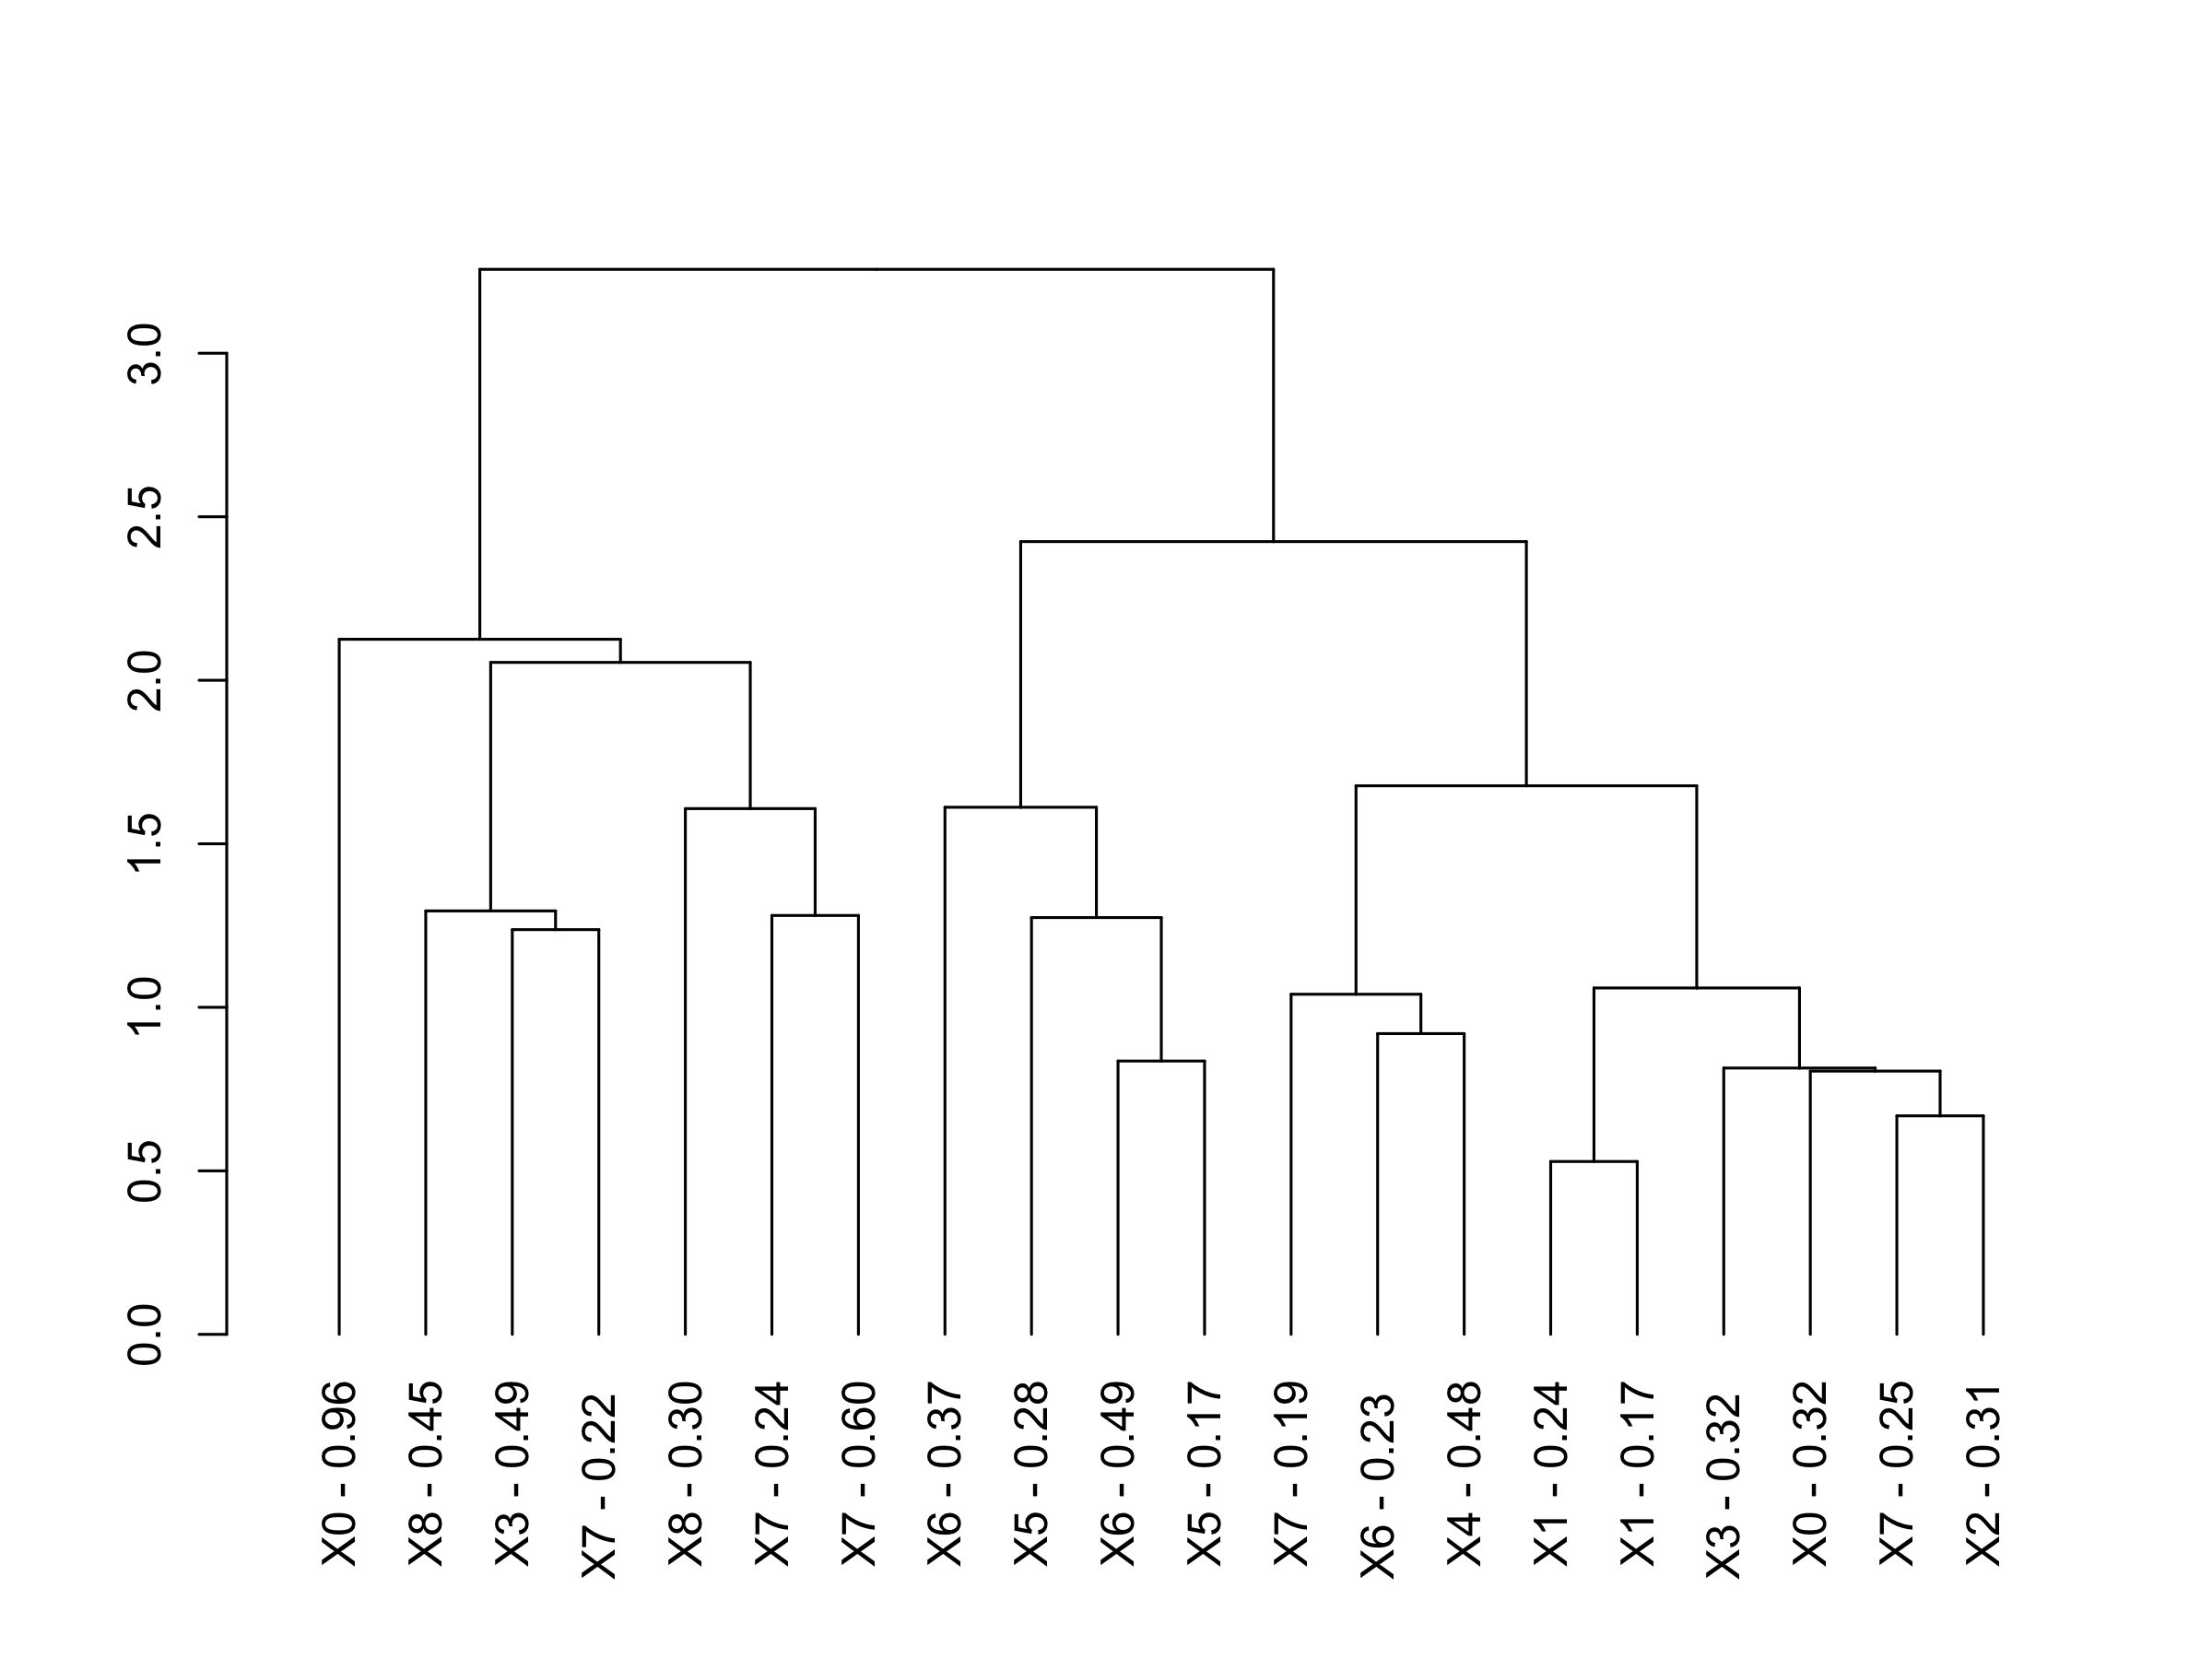
\includegraphics[width = 0.7\textwidth]{dendogram_data_class.png}\label{fig:1}} 
		 		\end{figure}																						
		\missingfigure{confusionmatrix}			
		\todo{Insert some text}
\end{document}